%%%%%%%%%%%%%%%%%%%%%%% file template.tex %%%%%%%%%%%%%%%%%%%%%%%%%
%
% This is a general template file for the LaTeX package SVJour3
% for Springer journals.          Springer Heidelberg 2010/09/16
%
% Copy it to a new file with a new name and use it as the basis
% for your article. Delete % signs as needed.
%
% This template includes a few options for different layouts and
% content for various journals. Please consult a previous issue of
% your journal as needed.
%
%%%%%%%%%%%%%%%%%%%%%%%%%%%%%%%%%%%%%%%%%%%%%%%%%%%%%%%%%%%%%%%%%%%
%
% First comes an example EPS file -- just ignore it and
% proceed on the \documentclass line
% your LaTeX will extract the file if required
\begin{filecontents*}{example.eps}
%!PS-Adobe-3.0 EPSF-3.0
%%BoundingBox: 19 19 221 221
%%CreationDate: Mon Sep 29 1997
%%Creator: programmed by hand (JK)
%%EndComments
gsave
newpath
  20 20 moveto
  20 220 lineto
  220 220 lineto
  220 20 lineto
closepath
2 setlinewidth
gsave
  .4 setgray fill
grestore
stroke
grestore
\end{filecontents*}
%
\RequirePackage{fix-cm}
%
%\documentclass{svjour3}                     % onecolumn (standard format)
%\documentclass[smallcondensed]{svjour3}     % onecolumn (ditto)
\documentclass[smallextended]{svjour3}       % onecolumn (second format)
%\documentclass[twocolumn]{svjour3}          % twocolumn
%
\smartqed  % flush right qed marks, e.g. at end of proof
%
\usepackage{amsmath}
\usepackage{amssymb}
\usepackage{bm}
\usepackage{graphicx}
\usepackage{epstopdf}
\usepackage{algorithm}
\usepackage[noend]{algpseudocode}
\usepackage[round]{natbib}
\usepackage{multirow}
\usepackage{pgfplots}
\usepackage{tikz}
\usepackage{lscape}
\usepackage{caption}
\usepackage{siunitx}
\usepackage{booktabs}
% \usepackage[capitalize]{cleveref}
\usetikzlibrary{bayesnet}
\setcitestyle{aysep={ }} %Author-Year Separator
%
% \usepackage{mathptmx}      % use Times fonts if available on your TeX system
%
% insert here the call for the packages your document requires
%\usepackage{latexsym}
% etc.
%
% please place your own definitions here and don't use \def but
% \newcommand{}{}
%
% Insert the name of "your journal" with
% \journalname{myjournal}
%

%%%%%%%%%%%%%%%%%%%%%%%%%%%%%%%%%%%%%%%%%%%%%%%%%%%%%%%%%
% CUSTOM COMMANDS

\newcommand{\bigo}{\mathcal{O}} % NOTE(tim): if you prefer normal O change it here.

\newcommand{\paren}[1]{\mathopen{}\mathclose\bgroup\left(#1\aftergroup\egroup\right)}
\newcommand{\brock}[1]{\mathopen{}\mathclose\bgroup\left[#1\aftergroup\egroup\right]}
\newcommand{\curly}[1]{\mathopen{}\mathclose\bgroup\left\{#1\aftergroup\egroup\right\}}
\newcommand{\anglebrackets}[1]{\langle #1 \rangle}
\newcommand{\ceil}[1]{\lceil #1 \rceil}
\newcommand{\floor}[1]{\lfloor #1 \rfloor}

\newcommand{\discset}{\mathcal{M}}

\DeclareMathOperator*{\argmin}{arg\,min}
\DeclareMathOperator*{\argmax}{arg\,max}

\newcommand{\todo}[1]{\textcolor{magenta}{#1}}
\newcommand{\tim}[1]{\textit{\textcolor{blue}{#1}}}
\newcommand{\mykel}[1]{\textit{\textcolor{cyan}{#1}}}

%%%%%%%%%%%%%%%%%%%%%%%%%%%%%%%%%%%%%%%%%%%%%%%%%%%%%%%%%

\begin{document}

\title{Learning Discrete-valued Bayesian Networks from Mixed Data%\thanks{Grants or other notes
%about the article that should go on the front page should be
%placed here. General acknowledgments should be placed at the end of the article.}
}
%\subtitle{Do you have a subtitle?\\ If so, write it here}

%\titlerunning{Short form of title}        % if too long for running head

\author{Yi-Chun Chen           \and
        Tim A. Wheeler         \and
        Mykel J. Kochenderfer
}

%\authorrunning{Short form of author list} % if too long for running head

\institute{F. Author \at
              first address \\
              Tel.: +123-45-678910\\
              Fax: +123-45-678910\\
              \email{fauthor@example.com}           %  \\
%             \emph{Present address:} of F. Author  %  if needed
           \and
           S. Author \at
              second address
}

\date{Received: date / Accepted: date}
% The correct dates will be entered by the editor


\maketitle

\begin{abstract}
\todo{
Insert your abstract here. Include keywords, PACS and mathematical
subject classification numbers as needed.
}
\keywords{Discretization \and Bayesian Network \and Continuous Variable}
% \PACS{PACS code1 \and PACS code2 \and more}
% \subclass{MSC code1 \and MSC code2 \and more}
\end{abstract}

%%%%%%%%%%%%%%%%%%%%%%%%%%%%%%%%%%%%%%%%%%%%%%%%%%%%%%%%%%%%%%%%%%%%%%%%%%%%%%%%%%%%%%

\section{Introduction}
\label{intro}
Bayesian networks \citep{Pearl_1988, PGM_2009} are an increasingly popular method for modeling uncertainty and causality in science and engineering. They provide an efficient factorization of the joint probability distribution over a set of random variables. Bayesian networks first emerged from artificial intelligence research and have been applied to a wide variety of problems, ranging from decision-making systems \citep{DMU_2015}\mykel{better to use a primary source} to medical diagnoses \citep{Lustgarten_2011}. In most cases, we assume that all random variables in Bayesian networks are discrete, since many Bayesian network learning algorithms are unable to deal with continuous variables efficiently. However, many applications
require the use of continuous variables, such as position and velocity in dynamic systems \mykel{cite Kochenderfer JGCD article on encounter modeling}.

There are two common approaches to extending Bayesian networks to continuous variables.
The first is to model the conditional probability density of each continuous variable using specific families of parametric distributions, and then to redesign Bayesian network learning algorithms based on their parameters.
One successful example is belief propagation in Gaussian graphical models \citep{Weiss_2011}.
For other parametric distributions \citep{Ihler_2009} and non-linear functions~\todo{[cite]}, these redesigned algorithms are computationally expensive and do not perform well.
\mykel{$\bigstar$ We need to discuss this; talk about algorithms for inference and structure learning, expectation propagation, Gibbs, BVGS}

The second approach is discretization.
Automated discretization methods have been studied in machine learning and statistics for many years \citep{Dougherty_1995, Kerber_1992, Holte_1993, Fayyad_1993}, primarily for classification problems.
They search for the best discretization policy of a continuous attribute by considering its interation with the target class variable.
Interations and dependencies between variables in Bayesian networks are more complicated, where discretization requires considering the impact on the variable's Markov blanket.
Prior work exists for discretizing continuous variables in naive Bayesian networks and tree-augmented networks \citep{Fried_naive}, but only a few discretization methods for general Bayesian networks have been proposed \citep{Friedman_1996, Kozlov_1997, Monti_1998, Steck_2007}.

This paper describes a new Bayesian discretization method for continuous variables in Bayesian networks, extending prior work on single-variable discretization methods from \citet{Boulle_2006} and \citet{Lustgarten_2011}.
The proposed method optimizes the discretization policy relative to the network and takes parents, children, and spouse variables into account.
The optimal single-variable discretization method is derived in Section \ref{sec:single_var}, and a second heuristic method is proposed which reduces the runtime from exponential to polynomial.
Section \ref{sec:multi_var} covers Bayesian networks with multiple continuous variables and discretization while simultaneously learning network structure.
The paper concludes with a comparison against the existing minimum-description length \citep{Friedman_1996} method on real-world datasets in Section \ref{sec:experiments}.

%%%%%%%%%%%%%%%%%%%%%%%%%%%%%%%%%%%%%%%%%%%%%%%%%%%%%%%%%%%%%%%%%%%%%%%%%%%%%%%%%%%%%%

\section{Related Work}
\label{sec:related_work}
This section reviews the minimum description length (MDL) principle discretization \citep{Friedman_1996} and MODL discretization \citep{Boulle_2006} methods.
The former is the predominant discretization method for continuous variables in Bayesian networks, and is compared to our proposed method in Section \ref{sec:experiments}.
The latter is a discretization method for one continuous variable against a discrete target class, which our proposed method generalizes to Bayesian networks.
The asymptotical equivalence between MDL and MODL was examined in \citep{VL_2000}.

\subsection{MDL Discretization}
The MDL principle was first proposed by \cite{MDL_1978} and states that the best model for a dataset is one that minimizes the amount of information needed to describe it \citep{Grunwald_2009}.
MDL methods trade off goodness-of-fit against model complexity to reduce generalization error.
In the context of Bayesian networks, \cite{Friedman_1996} applied the MDL principle to determine the optimal number of discretization intervals for continuous variables and the optimal positions of their discretization boundaries.
Their approach selects a discretization policy that minimizes the sum of the description lengths of the discretized Bayesian network and the information necessary for recovering the continuous values from the discretized data.
For a Bayesian network with a single continuous variable $X$, the objective function is

% \begin{small}
\begin{equation}
\begin{aligned}
\frac{1}{2} \log(N) \left\lbrace  \lvert \Pi_{X_i} \rvert (\lvert X^*_i \rvert - 1) +
 {\sum_{j,X_i \in \Pi_{X_i}}} \lvert \Pi_{X^*_j} \rvert (\lvert X_j \rvert - 1) \right\rbrace + \log(\lvert {X^*_i} \rvert) \\
 + (N_i-1) H \left( {{|X^*_i| - 1}\over{N_i -1}}  \right) -N \cdot \left[ I(X^*_i,\Pi_{X_i}) + {\sum_{j,X_i \in \Pi_{X_i}}} I(X_j, \Pi_{X^*_j}) \right],
\end{aligned}
\end{equation}
% \end{small}

\mykel{$\bigstar\Pi_{X_i}$ is not defined until later}
\tim{$\Pi_{X_i}$ may be confusing with our use of $\prod_{i=1}^n$ later on.}

\noindent
% $I(\boldsymbol{A},\boldsymbol{B}) =  \sum_{\boldsymbol{a},\boldsymbol{b}} \hat{P}_D (\boldsymbol{a},\boldsymbol{b}) \log {{\hat{P}_D (\boldsymbol{a},\boldsymbol{b})}\over{\hat{P}_D (\boldsymbol{a}),\hat{P}_D (\boldsymbol{b})}}$
where $I(A,B)$ is the mutual information between the discrete variables $A$ and $B$, ${H(p) = -p \log(p) - (1-p) \log(1-p)}$ \tim{does $H(p)$ have a name? Entropy?}, $|A|$ is the cardinality of a discrete variable $A$, and $X^*_i$ is the discretized version of the $i$th sample of $X$.
\tim{What are $N$, and $N_i$?}
The optimal discretization policy can be found with dynamical programming.
For Bayesian networks with multiple continuous variables, the algorithm is applied to one variable at a time iteratively over all continuous variables.
While iterating, only one variable is treated as continuous and other continuous variables are discretized based on an initial discretization policy or the discretization result from a previous iteration.

The network structure is not always known in advance. Bayesian network structure learning can be extended to distributions including continuous variables by alternating between traditional discrete structure learning and optimal discretization. Starting with some preliminary discretization policy, one applys a structure learning algorithm to identify the locally optimal graph structure. The discretization policy is refined based on the learned network. The cycle is continued until convergence.

% The discretization technique proposed by \citet{Friedman_1996} is the most well-known of these methods. It is based on the minimum description length principle (MDL): the optimal discretization policy minimizes the description length of the Bayesian network and discretization policy. The MDL algorithm has an $\bigo\paren{N^3 + \paren{n_c {v_\text{max}}^{(n_c^p)_\text{max}} + {v_\text{max}}^{n_p}} \cdot N^2}$ runtime on Bayesian networks with a single continuous variable and multiple discrete variables, where $N$ is the number of data samples from the joint distribution, $n_p$ and $n_c$ are the numbers of parent and children variables for the continuous variable, $v_\text{max}$ is the largest cardinality over all variables in the Markov blanket, and  ${(n_c^p)_\text{max}}$ is the largest number of parent variables of the continuous variable's children. The MDL method iterates over all continuous variables until convergence in the case of multiple continuous variables, converging in a few cycles according to our tests of real-world data. Unfortunately, MDL tends to produce discrete variables with low cardinality~\todo{[cite]}\mykel{don't like low-cardinality. Maybe 'intervals' or something instead}.

\subsection{MODL Discretization}
MODL discretization \citep{Boulle_2006} is a Bayesian method for discretizing a continuous feature according to a class variable. Bayesian methods maximize the probability of the model given the data, $P(\textit{Model} \mid \textit{Data})$. An application of Bayes' rule and constant $P(\textit{Data})$ shows that this is equivalent to maximizing:
\begin{align}
P(\textit{Model}) \cdot P(\textit{Data} \mid \textit{Model})\text{,}
\end{align}

\noindent
where $P(\textit{Model})$ is a prior over models and ${P(\textit{Data} \mid \textit{Model})}$ is the data likelihood.
The data likelihood usually increases with the number of discretization intervals, as more intervals allow for richer representations.
The prior decreases as the number of discretization intervals increases to favor simpler models and prevent overfitting.
Maximizing ${P(\textit{Model}) \cdot P(\textit{Data} \mid \textit{Model})}$ requires a trade-off when determining the number of discretization intervals.

The MODL method uses dynamic programming to find the optimal discretization policy, and has an $\bigo\paren{N^3 + |\text{Class}| \cdot N^2}$ runtime, where $N$ is the of number of data instances.
\cite{Lustgarten_2011} suggest several formulations for the prior term $P(\text{Model})$.
Under a uniform prior probability over discretizations the runtime can be reduced to $\bigo\paren{|\text{Class}| \cdot N^2}$ without sacrificing optimality.

%%%%%%%%%%%%%%%%%%%%%%%%%%%%%%%%%%%%%%%%%%%%%%%%%%%%%%%%%%%%%%%%%%%%%%%%%%%%%%%%%%%%%%

\section{Preliminaries}
\label{sec:preliminaries}
This section provides a brief overview of Bayesian networks, including the factorization of joint probability distributions, sampling from a Bayesian network, and structure learning. These concepts will be used in later sections. The formal definition of a discretization policy for a continuous variable is also given.

\subsection{Bayesian Networks and Structure Learning}

\mykel{This all needs to be explained better. Too many variables are being defined at once.}
A Bayesian network $B$ is defined by a pair $(G,\Theta)$, where $G = (X,E)$ is a directed acyclic graph whose nodes correspond to a set of random variables $X = \brock{X_1, X_2, \ldots, X_n}$, and whose edges $E$ represent probabilistic dependencies among nodes.
The graph structure $G$ encodes the Markov property: each node $X_i$ is independent of its non-descendants given its parents $\Pi_{X_i}$ in $G$.
The conditional relations are parameterized by the elements of $\Theta$, which take the form $\theta_{x_i \mid \Pi_{x_i}} = P(x_i \mid \Pi_{x_i})$ for each possible value $x_i$ of $X_i$, and $\Pi_{x_i}$ of $\Pi_{X_i}$. The joint distribution over $X$ factors according to the Markov property:

\begin{equation}
P_B (X_1 , \ldots, X_n) = \prod_{i=1}^{n} P_B (X_i \mid \Pi_{X_i}) = \prod_{i=1}^{n} \theta_{x_i \mid \Pi_{x_i}}\text{.}
\end{equation}

Forward sampling is used to draw samples from the joint distribution represented by a Bayesian network.
Variables are sampled in topological order such that parental instantiations are always known~\citep[see][chap.~22]{algo_2009}.
\mykel{I think this ref is just for the topological sort; for sampling, cite DMU or PGM}
Furthermore, the parent $\rightarrow$ child sampling order can be reversed if the marginal probability of the child variable is known.
By Bayes' rule,

\begin{equation}
P(X_i \mid \Pi_{X_i}) \cdot \prod_{j = 1}^{ Pa( X_i)} P( \brock{\Pi_{X_i} }_j) = P(X_i) \cdot P(\Pi_{X_i} \mid X_i),
\end{equation}

\noindent
where $Pa(X_i)$ is the number of parents of $X_i$ and $\brock{\Pi_{X_i}}_j$ is the $j$th parent of $X_i$.
\mykel{this may be messed up. Maybe use DMU notation?}
% One can first sample $X_i$ by $P(X_i)$, then sample all the parent variables simultaneously by $P(\Pi_{X_i} \mid X_i)$. That is to say, $X_i$ becomes the starting point of sampling.

It is often necessary to infer the structure of a Bayesian network from data.
Three common approaches to Bayesian network structure learning are constraint-based, score-based, and Bayesian model averaging \citep[see][chap.~18]{PGM_2009}. This work uses the K2 structure learning algorithm \citep{K2}, one of the most successful score-based structure learning methods.
Score-based structure learning methods over discrete variables commonly evaluate candidate structures according to their likelihood, $\prod_i f(X_i, \Pi_{X_i})$, where

\begin{align}
f(X_i, \Pi_{X_i}) = \prod_{j=1}^{|\Pi_{X_i}|} {{(|X_i|-1)!}\over{(N_{ij} + |X_i|-1)!}} \prod_{k=1}^{|X_i|} \alpha_{ijk}!\text{,}
\end{align}

\noindent
where $|X_i|$ is the cardinality of $X_i$, $|\Pi_{X_i}|$ is number of possible instantiations of the parent variables of $X_i$, $\alpha_{ijk}$ is the number of instances of the $k$th value of $X_i$ with the $j$th parental instantiation, and $N_{ij} = \sum_{k=1}^{|X_i|} \alpha_{ijk}$.
The optimal structure is the most probably structure given the data.
The space of acyclic graphcs is superexponential in the number of nodes so it is common to rely on heuristic search strategies \citep{PGM_2009}.

The K2 algorithm assumes a topological ordering of variables and greedily adds parents to nodes to maximally increase the likelihood score.
A fixed ordering ensures acyclicity but does not guarantee a globally optimal network structure.
K2 is typically run multiple times with random variable orderings and the network with the highest likelihood is retained.

\subsection{Discretization Policies}

\tim{We need to adopt the same notation everywhere; $C$ should be a child, not a continuous variable}.
A discretization policy $M_C = \anglebrackets{t_1 < t_2 < \ldots < t_{k-1}}$ for a continuous variable $C$ is a mapping from $\mathbb{R}$ to $\brock{1,2,3,\ldots,k}$ such that
\begin{equation}
  M_C (x)=\begin{cases}
    1, & \text{if $x<t_1$}.\\
    i, & \text{if $t_{i-1} \leq x < t_i$}\text{.}\\
    k, & \text{if $t_{k-1} \leq x$}
  \end{cases}
\end{equation}

\noindent
The policy discretizes the continuous variable $C$ into $k$ intervals.
The discretization edges $t_{1:k-1}$ are restricted to the midpoints between two sorted instances of $C$.
An integer representation of $M_C$ can be obtained by sorting the samples of $C$ in an increasing order, $\curly{c_1,c_2,\ldots,c_N}$, and if $t_i = (c_{s_{i}} + c_{s_{i}+1})/2$ for $i=1,2,\ldots,k$, then $M_C = \anglebrackets{t_1,t_2, \ldots, t_{k-1}} \equiv \brock{n_1,n_2,..n_k}$, where $n_1 = s_1$ and $n_i = s_{i} - s_{i-1}$.
\mykel{Where did $s_i$ come from?}

%%%%%%%%%%%%%%%%%%%%%%%%%%%%%%%%%%%%%%%%%%%%%%%%%%%%%%%%%%%%%%%%%%%%%%%%%%%%%%%%%%%%%%

\section{Single Variable Discretization}
\label{sec:single_var}

This section covers discretization of a single continuous variable $X$ in a Bayesian network where all other variables are discrete.
Let $n_p$ and $n_c$ respectively refer to the number of parents and number of children of $X$.
Each child $C_i$ of $X$ may possess other parents, referred to as spouses of $X$.
The set of spouses of $X$ is denoted $\boldsymbol{S_i}$.

Let $D$ be a dataset of $N$ samples from which the discretization will be learned, sorted in ascending order according to $X$.
Let $D_{\boldsymbol{Y}}$ will refer to the data instances associated with variables $\boldsymbol{Y}$, thus $D_X = \{ x_1,x_2,x_3,\ldots,x_N \}$.
In order to facilitate understanding, we temporarily assume all values in $D_X$ are unique, that is, $x_1 < x_2 < \ldots < x_N$.
It follows that a discretization policy $M$ on $X$ can be written as $M_X = \brock{n_1,n_2,\ldots,n_k}$, where $k$, $n_1$, $n_2$, $\ldots,n_k$ are positive integers satisfying $N = \sum_{i=1}^k n_i$.
\mykel{$\bigstar$ This conflicts with Section 3.2, right?}
An optimal discretization policy maximizes $P(M)\cdot P(D\mid M)$ for some prior $P(M)$ and likelihood $P(D\mid M)$.

%Furthermore, since there might have repeated values for $D_x$, we assume there are $N'$ unique values of $D_x$ and $N' \leq N$. Note that the allowable discretization edges happens between two consective values of non-repeated value of $D_x$. For example, if $D_X = \{ 1.0,1.0,2.0\}$, then the only possible discretization edge is on $1.5$.


\subsection{Priors and Objective Function}

The following four principles for the optimal discretization policy, motivated by MODL, enable the formulation of $P(M)$ and $P(D \mid M)$:
\begin{enumerate}
\item A discretization edge located at $(x_i + x_{i+1})/2$ has probability
\begin{equation}
1 - {\exp(- L \cdot {{x_{i+1} - x_i}\over{x_N - x_1}})},
\end{equation}
where $L$ is the largest cardinality number of discrete variables in $X$'s Markov blanket. \tim{Where does this come from? Is there an intuitive explanation?}\mykel{$\bigstar$}
\item For a given interval of $M$, every distribution of $\Pi_X$ is equiprobable.
\item For each pair of $(C_i,\boldsymbol{S_i})$ and a given interval of $M$, every distribution of $C_i$ with a value of $\boldsymbol{S_i}$ is equiprobable.\mykel{$\bigstar$}
\item The distributions of each $C_i$ and $\Pi_X$ in each interval of $M$ with each value of $\boldsymbol{S_i}$ are independent from each other.\mykel{$\bigstar$}
\end{enumerate}

From the first principle one obtains
\begin{equation}
\label{eq:p_M}
P(M) = \prod_{i=1}^k \curly{ \brock{1 - {\exp(- L \cdot {{x_{s_i+1} - x_{s_i}}\over{x_N - x_1}})}} \cdot \exp\paren{L \cdot {{x_{s_{i}} - x_{s_{i-1} + 1}}\over{x_N - x_1}}}},
\end{equation}

\noindent
where $s_i = \sum_{j=1}^k n_j$ and $s_k = N$, $s_0 = 0$.
The Bayesian network graph structure causes the likelihood term $P(D \mid M)$ to factorizes according to $X$'s Markov blanket:

\begin{equation}
\label{eq:p_D_given_M}
P\paren{D \mid M} \propto P\paren{D_{\Pi_x} \mid M} \cdot \prod_{i = 1}^{n_c} P\paren{D_{C_i} \mid M, D_{\boldsymbol{S_i}}}\text{.}
\end{equation}

For example, in Figure 1., the corresponding $P(D \mid M)$ is factorized according to
\begin{equation}
P\paren{D_{ P_1,P_2,P_3 } \mid M} \cdot P\paren{ D_{ C_1 } \mid M,D_{\boldsymbol{S_1}}} \cdot P\paren{D_{C_2} \mid M,D_{ S_2  }}\text{.}
\end{equation}

\begin{figure}[ht]
    \begin{tabular}{cc}
      % model_pca.tex
%
% Copyright (C) 2012 Jaakko Luttinen
%
% This file may be distributed and/or modified
%
% 1. under the LaTeX Project Public License and/or
% 2. under the GNU General Public License.
%
% See the files LICENSE_LPPL and LICENSE_GPL for more details.

% PCA model

%\beginpgfgraphicnamed{model-pca}
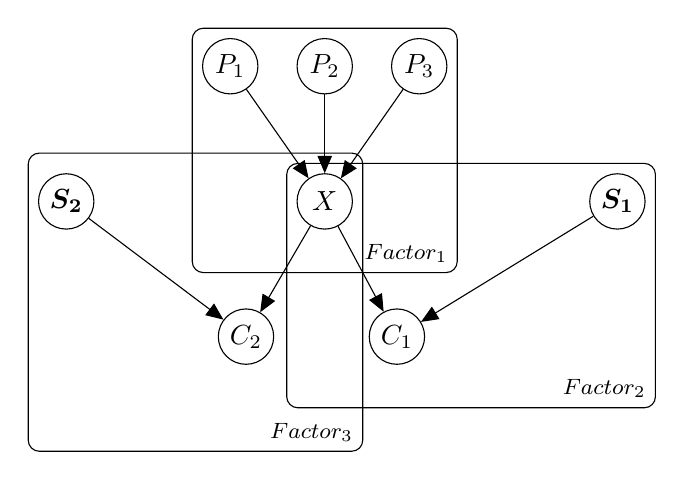
\begin{tikzpicture}

  % Define nodes
  \node[latent]                               (c1) {$C_2$};
  \node[latent, right= 1.2 cm of c1]            (c2) {$C_1$};
  \node[latent, above=of c1, xshift= 1 cm] (y)  {$X$};
  \node[latent, above=of y, xshift=-1.2cm] (p1) {$P_1$};
  \node[latent, above=of y, xshift=0cm]  (p2) {$P_2$};
  \node[latent, above=of y, xshift=1.2cm]  (p3) {$P_3$};
  \node[latent, right= 3.0cm of y]            (s1) {$\boldsymbol{S_1}$};
  \node[latent, right=-4.0cm of y]            (s2) {$\boldsymbol{S_2}$};

  % Connect the nodes
  \edge {p1,p2,p3} {y} ; %
  \edge {y,s1}{c2} ;
  \edge {y,s2}{c1};

  % Plates
  \plate {} {(p1)(p2)(p3)(y)} {$Factor_1$} ;
  \plate {yx} {(y)(s1)(c2)} {$Factor_2$};
  \plate {} {(y)(s2)(c1)(yx.north west)(yx.south west)} {$Factor_3$} ;
  %\plate {} {(w)(y)(yx.north west)(yx.south west)} {$M$} ;

\end{tikzpicture}
%\endpgfgraphicnamed

%%% Local Variables: 
%%% mode: tex-pdf
%%% TeX-master: "example"
%%% End: 

    \end{tabular}
  \caption{Factorization of $P(D \mid M)$}
\end{figure}


The concept behind the factorization also the motivation behind forward sampling in a Bayesian network.
The parents of $X$ are independent of the children given $X$.
The parents are not necessarily individually independent, and thus the parental term $P(D_{\Pi_x} \mid M)$ cannot be factored further.
The children of $X$ are similarly independent given $X$ and its spouses $\boldsymbol{S_i}$, leading to their factored product $\prod_{i = 1}^{n_c} P(D_{C_i} \mid M, D_{\boldsymbol{S_i}})$.
Each component in the decomposition be evaluated based on a discretization policy $M = [n_1,n_2,\ldots,n_k]$ and dataset $D$.

\subsubsection{Evaluation of $P(D_{\Pi_x} \mid M)$}
Let $J_P = \prod_{i=1}^{n_p} \| P_i \|$. It follows that

\begin{equation}
\label{eq:likelihood_one}
P(D_{\Pi_X} \mid M) = \prod_{i=1}^k  {{1}\over{{n_i + J_P - 1}\choose{J_P -1}}}
{{1}\over{ {{{n}_i}!}\over{ {n^{(p)}_{i,1} !} {n^{(p)}_{i,2} !} \cdots {n^{(p)}_{i,J_P} !}}  }}\text{,}
\end{equation}

\noindent
where $n^{(p)}_{i,j}$ is the number of instances in the $i$th discretized interval with the $j$th value of $\Pi_X$.
Note that $n_i = \sum_{j=1}^{\| \Pi_x \|} n^{(p)}_{i,j}$.
The two factors on the right hand side comes from the second prior: all distributions of values of $\Pi_X$ in a given interval are equiprobable. According to the fourth prior, the distribution in each interval is independent, so the two factors are multiplied together.

\subsubsection{Evaluation of $P(D_{C_i} \mid M, D_{\boldsymbol{S_i}})$}
For each pair $(C_j, \boldsymbol{S_j})$, let $\|C_j \| = J_j$ and $\| \boldsymbol{S_j} \| = L_j = \prod_{v \in \boldsymbol{S_j}} \| v \|$. It follows that

\begin{equation}
\label{eq:likelihood_two}
P(D_{C_j}  \mid M, D_{S_j}) =
\prod_{i=1}^{k} \prod_{l=1}^{L_j} {{1}\over{{n_{i,l} + J_j - 1}\choose{J_j-1}}}
{{1}\over{ {{n_{i,l}}!}\over{ {n^{(j)}_{i,1,l} !} {n^{(j)}_{i,2,l} !} \cdots {n^{(j)}_{i,J_j,l} !}}  }}\text{,}
\end{equation}

\noindent
where $n^{(j)}_{i,m,l}$ is the number of instances in $i$th interval with $m$th value of $C_j$ and $l$th value of $\boldsymbol{S_j}$, $n_{i,l} = \sum_{m=1}^{J_j} n^{(j)}_{i,m,l}$, and $n_i = \sum_{l=1}^{L_j} n_{i,l}$.
The two factors on the right hand side come from the third prior: all distribution of values of $C_j$ in a given interval and with a given value of $S_j$ are equiprobable. According to the forth prior, these distributions are independent from each other, and one thus takes their product. If $S_j = \emptyset$, then Equation~\ref{eq:likelihood_two} is equivalent to

\begin{equation}
\label{eq:likelihood_three}
P(D_{C_j}  \mid M) =
\prod_{i=1}^{k}  {{1}\over{{n_{i} + J_j - 1}\choose{J_j-1}}}
{{1}\over{ {{n_{i}}!}\over{ {n^{(j)}_{i,1,\emptyset} !} {n^{(j)}_{i,2,\emptyset} !} \cdots {n^{(j)}_{i,J_j,\emptyset} !}}  }}\text{,}
\end{equation}

\noindent
where $n^{(j)}_{i,m,\emptyset}$ is the number of instances in the $i$th interval with the $m$th value of $C_j$, and $\sum_{m=1}^{J_j} n^{(j)}_{i,m,\emptyset} = n_i$.

The objective function can be formulated given equations \ref{eq:p_M}, \ref{eq:p_D_given_M}, \ref{eq:likelihood_one}, and \ref{eq:likelihood_three}.
The log-inverse of $P(M) \cdot P(D|M)$ is minimized for computational convenience:

\begin{equation}
\label{eq:opt_prob}
\begin{aligned}
& \sum_{i=1}^{k-1} - \log(1 - {\exp(- L \cdot {{x_{s_i+1} - x_{s_i}}\over{x_N - x_1}})}) +  \sum_{i=1}^{k} L \cdot {{x_{s_{i}} - x_{s_{i-1} + 1}}\over{x_N - x_1}} +\\
&  \sum_{j=1}^{n_c} \sum_{i=1}^{k}  \sum_{l=1}^{L_j} \left[  \log{{n_{i,l} + J_j - 1}\choose{J_j-1}} + \log \left( { {{n_{i,l}}!}\over{ {n^{(j)}_{i,1,l} !} {n^{(j)}_{i,2,l} !} \cdots {n^{(j)}_{i,J_j,l} !}} } \right) \right] + \\
& \sum_{i=1}^k \left[  \log {{n_{i} + J_P - 1}\choose{J_P-1}} + \log \left( { {{n_i}!}\over{ {n^{(p)}_{i,1} !} {n^{(p)}_{i,2} !} \cdots {n^{(p)}_{i,J_p} !}} } \right) \right]\text{.}
\end{aligned}
\end{equation}

All parameters and variables in the objective function are explained in previous subsections.

\subsection{Algorithm}

This section describes the procedure used to minimize the objective function.
Note that the objective function is cumulative over intervals, thus, if a partition of $X$ into $k$ intervals with lengths $n_1,n_2,\ldots,n_k$ is an optimal discretization policy, then any subinterval is optimal for the corresponding subproblem.
It follows that dynamic programming can be used to solve the optimization problem exactly.

Every midpoint between two nonequal consecutive values in $D_X$ is a candidate discretization edge.
Let ${D'_X} = \brock{x'_1,x'_2,\ldots,x'_M}$ be the set of unique values of $D_X$ sorted in ascending order, where $M$ is the number unique values in $D_X$.
Recall that $D_X$ is also sorted.
Let $b = \brock{b_0,b_1,b_2,\ldots,b_M}$ be an increasing sequence of integers marking the repeated value intervals in $D_X$ such that $b_0 = 0$ and $x_{b_{i-1} + 1} = x_{b_{i-1} + 2} = \ldots = x_{b_i} = x'_i$.
By this definition, the allowable discretization positions are $d_i = \paren{x_{b_{i}} + x_{{b_i}+1}}/2$ for all $i = 1,2,\ldots,M-1$.

Precomutation reduces runtime.
Compute $h(u,v)$ for each interval $I_q$ starting from $x_{u}$ to $x_{v}$ for all $(u,v)$ satisfying $u \leq v$:

\begin{small}
\begin{equation}
\begin{aligned}
h(u,v) &=  \log {{n_{q} + J_P - 1}\choose{J_P-1}} + \log \left( { {{n_q}!}\over{ {n^{(p)}_{q,1} !} {n^{(p)}_{q,2} !} \cdots {n^{(p)}_{q,J_p} !}} } \right) \\
& + \sum_{j=1}^{n_c} \sum_{l=1}^{L_j} \left[  \log{{n_{q,l} + J_j - 1}\choose{J_j-1}} + \log \left( { {{n_{q,l}}!}\over{ {n^{(j)}_{q,1,l} !} {n^{(j)}_{q,2,l} !} \cdots {n^{(j)}_{q,J_j,l} !}} } \right) \right]
\end{aligned}
\end{equation}
\end{small}

The evaluation of $h(u,v)$ for all $u \leq v$ is summarized in Algorithm \ref{alg:h} in the appendix.
The calculation has a $O(n_c  {v'_\text{max}} \cdot N^2 + {v'_\text{max}}^{n_p} \cdot N^2)$ runtime, where $n_c$ and $n_p$ are the numbers of child and parent variables respectively, and $v'_\text{max}$ is the largest cardinality of variables that directly connect to $X$.

Now we are able to solve the optimization problem over Equation~\ref{eq:opt_prob}.
The dynamic programming procedure is shown in Algorithm~\ref{alg:disc_one}.
It takes two inputs: $D$, the joint samples over all variables sorted in ascending order according to $D_X$, and $G$, the network structure.
The runtime of Algorithm \ref{alg:disc_one} is also $O(n_c  {v'_\text{max}} \cdot N^2 + {v'_\text{max}}^{n_p} \cdot N^2)$, because the runtime of the dynamic programming procedure is less than the runtime for computing $h(u,v)$.
Algorithm \ref{alg:disc_one} is guaranteed to be optimal.
For faster methods with suboptimal results please refer to \citep{Boulle_2006}.

\begin{algorithm}
\caption{Discretization of one continuous variable in a Bayesian network}
\label{alg:disc_one}
\begin{algorithmic}[5]
\Function{Discretize}{$D$, $G$}
\State
\State $N \leftarrow$ the number of instances
\State $N' \leftarrow$ the number of unique values in $D_X$
\State $H \leftarrow$ an $N \times N$ matrix such that $H[u,v] = h(u,v)$ per Algorithm \ref{alg:h} in the appendix
\State $b \leftarrow$ the increasing sequence of $M$ integers as previously defined
\State $L \leftarrow$ the largest cardinality over all discrete variables in the Markov blanket of $X$
\State $S[u] \leftarrow$ the optimal objective value of subproblems with instances from $1$ to $u$
\State $M[u] \leftarrow$ the optimal discretization for subproblems with instances from $1$ to $u$
\State $W[u]  \leftarrow - \log\brock{1 - {\exp\paren{- L \cdot{ {{x_{b(u)+1} - x_{b(u)}}\over{x_N - x_1}}}}}}$ for $u = 1,2, \ldots,N'-1$ and $L(N') \leftarrow 0$
\State
\For {$v = 1$ to $N'$}
\If {$v = 1$}
\State $S[v] \leftarrow g \left(1,b[v] \right) + L[v]$
\State $M[v] \leftarrow \{ ({x_{b[v]} + x_{b[v]+1}}) / 2\}$
\Else
\State $s \leftarrow \infty$ and $boundary \leftarrow \infty$
\For {$u = 1$ to $v$}
\State $s' \leftarrow S[u] + g \left( b[u]+1,b[v] \right) +  {L \cdot {{x_{b[v]} - x_{b[u] + 1}}\over{x_N - x_1}}} + W[v]$
\If {$s' < s$}
\State $s \leftarrow s'$
\State $boundary \leftarrow ({x_{b[u]} + x_{b[u]+1}}) / 2$
\EndIf
\EndFor
\State $S[v] \leftarrow s$
\State $M[v] \leftarrow M[u] \cup \{ boundary\}$
\EndIf
\EndFor
 \State \Return $M$
\EndFunction
\end{algorithmic}
\end{algorithm}


\subsection{Approximation}

Algorithm \ref{alg:disc_one} has an exponential $\bigo\paren{\paren{v'_\text{max}}^{n_p} \cdot N^2}$ runtime which severely limits discretization in networks with a large number of discretization intervals or parent variables.
This section introduces an approximation to the objective function that significantly reduces the runtime and still preserves the quality of discretization.
The approximation replaces the dominator of the last factor in Equation~\ref{eq:likelihood_one} with

\begin{equation}
{\frac{{n_i}!}{ {n^{(p)}_{i,1} !} {n^{(p)}_{i,2} !} \cdots {n^{(p)}_{i,J_P} !}}} \approx \prod_{r=1}^{n_p} { {{{n}_i}!}\over{ {n^{(p_r)}_{i,1} !} {n^{(p_r)}_{i,2} !} \cdots {n^{(p_r)}_{i,J_{p_r}} !}}}\text{,}
\end{equation}

\noindent
where $J_{p_r} = \| P_r\|$ and ${n^{(p_r)}_{i,j} !}$ is the number of instances in the $i$th interval with the $j$th value of $P_r$.
The approximated objective function is

\begin{small}
\begin{equation}
\begin{aligned}
\label{eq:opt_prob_approx}
& \sum_{i=1}^{k-1} - \log(1 - {\exp(- L \cdot {{x_{s_i+1} - x_{s_i}}\over{x_N - x_1}})}) +  \sum_{i=1}^{k} L \cdot {{x_{s_{i}} - x_{s_{i-1} + 1}}\over{x_N - x_1}} +\\
&  \sum_{j=1}^{n_c} \sum_{i=1}^{k}  \sum_{l=1}^{L_j} \left[  \log{{n_{i,l} + J_j - 1}\choose{J_j-1}} + \log \left( { {{n_{i,l}}!}\over{ {n^{(j)}_{i,1,l} !} {n^{(j)}_{i,2,l} !} \cdots {n^{(j)}_{i,J_j,l} !}} } \right) \right] + \\
& \sum_{i=1}^k \left[  \log {{n_{i} + J_P - 1}\choose{J_P-1}} + \sum_{q=1}^{n_p} \log \left( { {{{n}_i}!}\over{ {n^{(p_q)}_{i,1} !} {n^{(p_q)}_{i,2} !} \cdots {n^{(p_q)}_{i,J_{p_q}} !}}} \right) \right]\text{.}
\end{aligned}
\end{equation}
\end{small}

The approximation reduces the runtime of Algorithm~\ref{alg:disc_one} to a polynomial, $\bigo\paren{ {v'_\text{max}} \cdot (n_c + n_p) \cdot N^2}$.
It will be shown in Section~\ref{sec:experiments} that the approximation is more sensitive to the distribution over other variables and is biased towards slightly higher interval counts.
\tim{We need to have a more specific thing to say along the lines of When does it fail?}

With the approximated objective function, Equation~\ref{eq:opt_prob_approx}, provides intuition into how child and parent variables contribute to the objective function.
For example, in the left graph of Figure~\ref{fig:example_networks}, the corresponding square brackets in the approximated objective function are

\begin{small}
\begin{equation}
\begin{aligned}
\label{eq:example_approx}
 \sum_{i=1}^k & \left\lbrace   \left[ \log{{n_{i} + J_{C_1} - 1}\choose{J_{C_1}-1}} + \log \left(  {{{n_i}!} \over { {n^{(1)}_{i,1,\emptyset} !} \cdots {n^{(1)}_{i,J_{C_1},\emptyset} !}} }  \right)  +  \right. \right.\\
& \left.  \log{{n_{i} + J_{C_2} - 1}\choose{J_{C_2}-1}} + \log \left(  {{{n_i}!} \over { {n^{(2)}_{i,1,\emptyset} !} \cdots {n^{(2)}_{i,J_{C_1},\emptyset} !}} }  \right)  \right] + \\
&  \left. \left[  \log {{n_{i} + J_P - 1}\choose{J_P-1}} +  \log \left( { {{{n}_i}!}\over{ {n^{(p_1)}_{i,1} !}\cdots {n^{(p_1)}_{i,J_{p_1}} !}}} \right) +{ {{{n}_i}!}\over{ {n^{(p_2}_{i,1} !}\cdots {n^{(p_2)}_{i,J_{p_2}} !}}}  \right] \right\rbrace \text{.}
\end{aligned}
\end{equation}
\end{small}

In Equation~\ref{eq:example_approx}, each child carries two terms, as shown in the first set of square brackets, but the two parent variables only carry a total of three terms, as shown in the second set of square brackets.
In this case the child variables have greater effect than the parent variables even though the number of child and parent variables are the same.
However, if $C_2$ has an additional parent $S_2$, as shown in the right graph of Figure~\ref{fig:example_networks}, the importances of $C_2$ will be reduced, because the information from $C_2$ is now affected by $S_2$.
This argument shows that the proposed method, both before and after approximation, indeed incorporates graph structure when discretizing continuous variables.

\begin{figure}[ht]
  \centering
  \begin{tabular}{cc}
    % model_pca.tex
%
% Copyright (C) 2012 Jaakko Luttinen
%
% This file may be distributed and/or modified
%
% 1. under the LaTeX Project Public License and/or
% 2. under the GNU General Public License.
%
% See the files LICENSE_LPPL and LICENSE_GPL for more details.

% PCA model

%\beginpgfgraphicnamed{model-pca}
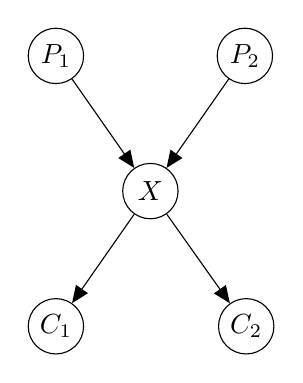
\begin{tikzpicture}

  % Define nodes
  \node[latent]                               (c1) {$C_1$};
  \node[latent, right= 1.7 cm of c1]            (c2) {$C_2$};
  \node[latent, above=of c1, xshift= 1.2 cm] (y)  {$X$};
  \node[latent, above=of y, xshift=-1.2cm] (p1) {$P_1$};
  \node[latent, above=of y, xshift=1.2cm]  (p2) {$P_2$};

  % Connect the nodes
  \edge {p1,p2} {y} ; %
  \edge {y} {c2} ;
  \edge {y}{c1};

  % Plates
  %\plate {} {(p1)(p2)(p3)(y)} {$Factor_1$} ;
  %\plate {yx} {(y)(s11)(s12)(c2)} {$Factor_2$};
  %\plate {} {(y)(s2)(c1)(yx.north west)(yx.south west)} {$Factor_3$} ;
  %\plate {} {(w)(y)(yx.north west)(yx.south west)} {$M$} ;

\end{tikzpicture}
%\endpgfgraphicnamed

%%% Local Variables: 
%%% mode: tex-pdf
%%% TeX-master: "example"
%%% End: 

    \end{tabular}
   \hspace{5em}
    \begin{tabular}{cc}
    % model_pca.tex
%
% Copyright (C) 2012 Jaakko Luttinen
%
% This file may be distributed and/or modified
%
% 1. under the LaTeX Project Public License and/or
% 2. under the GNU General Public License.
%
% See the files LICENSE_LPPL and LICENSE_GPL for more details.

% PCA model

%\beginpgfgraphicnamed{model-pca}
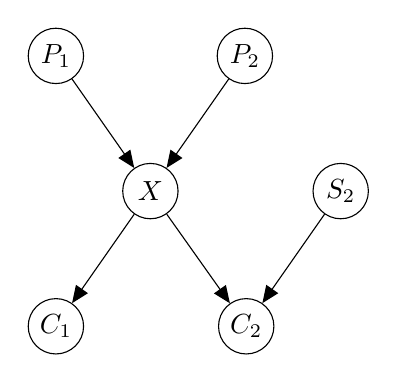
\begin{tikzpicture}

  % Define nodes
  \node[latent]                               (c1) {$C_1$};
  \node[latent, right= 1.7 cm of c1]            (c2) {$C_2$};
  \node[latent, above=of c1, xshift= 1.2 cm] (y)  {$X$};
  \node[latent, above=of c2, xshift= 1.2 cm] (s)  {$S_2$};
  \node[latent, above=of y, xshift=-1.2cm] (p1) {$P_1$};
  \node[latent, above=of y, xshift=1.2cm]  (p2) {$P_2$};

  % Connect the nodes
  \edge {p1,p2} {y} ; %
  \edge {y} {c2} ;
  \edge {y}{c1};
  \edge {s}{c2};

  % Plates
  %\plate {} {(p1)(p2)(p3)(y)} {$Factor_1$} ;
  %\plate {yx} {(y)(s11)(s12)(c2)} {$Factor_2$};
  %\plate {} {(y)(s2)(c1)(yx.north west)(yx.south west)} {$Factor_3$} ;
  %\plate {} {(w)(y)(yx.north west)(yx.south west)} {$M$} ;

\end{tikzpicture}
%\endpgfgraphicnamed

%%% Local Variables: 
%%% mode: tex-pdf
%%% TeX-master: "example"
%%% End: 

  \end{tabular}
  \caption{Two example networks}
  \label{fig:example_networks}
\end{figure}

%%%%%%%%%%%%%%%%%%%%%%%%%%%%%%%%%%%%%%%%%%%%%%%%%%%%%%%%%%%%%%%%%%%%%%%%%%%%%%%%%%%%%%

\section{Extension to Multiple Continuous Variables}
\label{sec:multi_var}

\subsection{Discretization of Multiple Continuous Variables}

The single-variable discretization method can be extended to Bayesian networks with multiple continuous variables by iteratively discretizing variables individually.
The discretization process for a single variable requires that all other variables be discrete.
The iterative approach thus requires a prediscretization policy from which to initialize the process.
This work uses prediscretization with equal-width intervals, defined by

\begin{equation}
M_X = \curly{X_\text{min}, X_\text{min} + \delta, X_\text{min} + 2\delta, \ldots, X_\text{max}}\text{,}
\end{equation}

\noindent
where $X_\text{min}$ and $X_\text{max}$ are the extrema values of $D_X$, $\delta = (X_\text{max} - X_\text{min})/k$, and $k$ is the desired number of intervals.
This work sets $k$ to the median value of the cardinalities of initially discrete variables in the network.
After prediscretization, the one-variable discretization methis is iteratively applied over each continuous variable in reverse topoligical order, from the leaves to the root.
Let one such series of discretizations be a cycle.
Reverse topological order has the advantage of using less prediscretized instantiations during the first cycle.
For example, in the right-hand graph of Figure \ref{fig:example_networks}, assume $S_2$ is the only discrete variable.
The discretization of $P_1$ involves both $P_2$ and $X$, whereas the discretization of $C_1$ only involves $X$.

The algorithm is terminated when the number of discretization intervals and their associated edges converge for all variables.
A maximum cycle count is enforced to prevent infinite iterations when convergence does not occur.
The algorithm typically converges within a few cycles when tested on real-world data.
In cases where it does not converge, ten cycles usually produce decent discretization results.

The pseudocode for the multi-variable discretization procedure is shown in Algorithm \ref{alg:disc_two}.
It requires four inputs: $D''$, the joint samples from all network variables; $G$, the network structure; $C$, the set of all continuous variables in a reverse topological order; and $u_{cycle}$, the upper bound of times of cycles.

\begin{algorithm}
  \label{alg:disc_two}
  \caption{Discretization of multiple continuous variables \todo{Fix label reference number}}
  \begin{algorithmic}[5]
  \Function{Discretize}{$D''$, $G$, $C$, $u_{cycle}$}
    \State
    \State $M[i] \leftarrow$ the discretization policy for the $i$th variable
    \State $n \leftarrow$ the number of variables in the Bayesian network
    \State $D^*_i \leftarrow M[i] (D_i)$, list of samples $D_i$ discretized according to $M[i]$
    \State $D^* \leftarrow $ the discretized data for all variables, where $D^*_i \leftarrow D''_i$ if $i \notin C$
    \State $k \leftarrow median\{ |v|, v\notin C\}$
    \State
    \For {$i = 1$ to $n$}
      \If {$i \in C$}
        \State $M[i] \leftarrow$  equal-width discretization with $k$ intervals
        \State $D^*_i \leftarrow  M[i] (D''_i)$
      \EndIf
    \EndFor
    \State
    \State $cycle \leftarrow 0$
    \While {$M$ is not converged  \textbf{and} $cycle \leq u_{cycle}$}
      \State {$cycle  \leftarrow cycle  + 1$}
      \For {$j = 1$ to $|C|$}
        \State $D^*_{\backslash C(j)} \leftarrow D^*$ without $D^*_{C(j)}$.
        \State {$M[C(j)] \leftarrow $ DISCRETIZE($D_{C(j)}$,$D^*_{ \backslash C(j)}$,graph)}
        \State {$D^*_{C(j)}  \leftarrow$ $M[C(j)](D''_{C(j)})$}
      \EndFor
    \EndWhile
    \State \Return $M$
  \EndFunction
  \end{algorithmic}
\end{algorithm}

\subsection{Combining Discretization with Structure Learning}

In many situations the network structure is not known in advance and must be learned from data.
Traditional Bayesian structure learning algorithms require discretized data, whereas the proposed discretization algorithm requires a network structure.
This section combines the proposed discretization method with the K2 structure learning algorithm \citep{K2} in an interative fassion to simultaneously perform Bayesian structure learning and discretization of continuous variables.

The proposed algorithm alternates between K2 structure learning and discretization.
K2 is run on the discretized dataset corresponding to prediscretizations for all continuous variables.
The affected continuous variables are rediscretized every time an edge is added by K2.
The resulting discretization policies are used to update the discretized dataset, and the next step of the K2 algorithm is executed.
This cycle is repeated until the K2 algorithm reaches a local maximum.

This procedure is given in Algorithm \ref{alg:structure_learn}.
It takes five inputs: $D'$, the joint samples from all network variables; $C$, the set of all continuous variables; $order$, the permutation of variable for $K2$; $u_{parent}$, the upper bound on the number of parents per node for $K2$; and $u_{cycle}$, the upper bound on the cycle count.
It is common practice to run K2 multiple times with different permutations of the variables and to then choose the structure with the highest score.
This work runs Algorithm \ref{alg:structure_learn} multiple times, each with a different order, and picks the discretized Bayesian network with the highest score.

\begin{algorithm}
  \label{alg:structure_learn}
  \caption{ Learning a discrete-valued Bayesian network}
  \begin{algorithmic}[5]
  \Function{Learn\_DBN}{$D''$, $C$, $order$, $u_{parent}$, $C$, $u_{cycle}$}
    \State $n \leftarrow$ the number of variables in the Bayesian network
    \State $k \leftarrow median\{ \|v\|, v\notin C\}$
    \State $M[i] \leftarrow$ the discretization policy for the $i$th variable
    \State $D^*_i \leftarrow M[i] (D_i)$, list of samples $D_i$ discretized according to $M[i]$
    \State $D^* \leftarrow $ the discretized data for all variables, where $D^*_i \leftarrow D''_i$ if $i \notin C$
    \State $G \leftarrow$ the initial edgeless graph structure
    \For {$i = 1$ to $n$}
      \If {$i \in C$}
        \State $M[i] \leftarrow$  equal-width discretization with $k$ intervals
        \State $D^*_i \leftarrow  M[i] (D''_i)$
      \EndIf
    \EndFor
    \For {$i =1$ to $n$}
      \State $P_{old} \leftarrow f(X^*_i,\Pi_{X^*_i})$: Equation~\ref{eq:f_x_p}
      \State OKToProceed $\leftarrow$ \textbf{true}
      \While {OKToProceed \textbf{and} $\|\Pi_{X^*_i}\| < u_{parent}$}
        \State $Y \leftarrow$ an element from the set $order[1:i] \backslash \Pi_X$
        \State $P_{new} \leftarrow f(X^*_i,\Pi_{X^*_i} \cup Y)$
        \If {$P_{new} > P_{old}$}
          \State $P_{old} \leftarrow P_{new}$
          \State $\Pi_{X_i} \leftarrow \Pi_{X_i} \cup Y $
          \State $M \leftarrow$ {DISCRETIZE}({$D''$, $G$, $C$, $u_{cycle}$}): Algorithm \ref{alg:disc_two}
          \State $D* = M(D'')$
        \Else
          \State OKToProceed $\leftarrow$ \textbf{false}
        \EndIf
      \EndWhile
    \EndFor
    \State \Return $G$, $M$
  \EndFunction
  \end{algorithmic}
\end{algorithm}

%%%%%%%%%%%%%%%%%%%%%%%%%%%%%%%%%%%%%%%%%%%%%%%%%%%%%%%%%%%%%%%%%%%%%%%%%%%%%%%%%%%%%%

\section{Experiments}
\label{sec:experiments}

This section describes experiments conducted to evaluate the proposed methods.
All experiments were run on datasets from the publically available Irvine machine learning repository \citep{Lichman:2013}.
Variables are labelled alphabetically in the order given on the dataset information webpage.
Subscripts inducate the number of discretized intervals.
Shaded nodes are originally discrete and unshaded nodes are originally continuous.

For each dataset, the experiment consists of two parts.
In the first part, the Bayesian network structure is known in advance, which is obtained by equal-width prediscretization and the K2 algorithm.
In the second part, the Bayesian netowrk structure is not provided in advance, and it is learned along with the discretization process.
\tim{We may not want to state this up front so we can modify what we show for each dataset.}

The discretizations are compared using the mean cross validated log-likelihood of the data set $D$ given the resulting graph structure $G$ and discretization policy set $\discset$.
The log-likelihood contains two components,

\begin{equation}
\ln p(D\mid G, \discset) = \ln P(D^*\mid G) + \ln p(D\mid \discset, D^*)\text{,}
\end{equation}

\noindent
where $D$ is the original dataset and $D^*$ is the dataset discretized according to $\discset$.
The log-likelihood of the discretized dataset is the Bayesian score evaluated with a uniform prior~\citep{neapolitan2004learning}:

\begin{equation}
  \ln P(D^*\mid G) = \sum_{i=1}^n \sum_{j=1}^{q_i} \ln\paren{
    \frac{
      \Gamma\paren{\alpha_{ij0}}
    }{
      \Gamma\paren{\alpha_{ij0} + m_{ij0}}
    }
  } + \sum_{k=1}^{r_i} \ln\paren{
    \frac{
      \Gamma\paren{\alpha_{ijk} + m_{ijk}}
    }{
      \Gamma\paren{\alpha_{ijk}}
    }
  }\text{.}
\end{equation}

\tim{We need to make sure everything is defined.}

The log-likelihood of the original dataset given the discrete dataset is

\begin{equation}
  \ln p(D\mid \discset, D^*) = \sum_{i=1}^n \sum_{j=1}^{q_i} \sum_{k=1}^{r_i} m_{ijk} \ln\paren{
    \frac{
      1
    }{
      \discset^{(ij)}_{k+1} - \discset^{(ij)}_{k}
    }
  }\text{.}
\end{equation}

\subsection{Auto MPG Dataset}

In this subsection, two experiments are conducted on the Auto MPG dataset from the Irvine repository \citep{Lichman:2013}.
The dataset has \num{392} instances after deleting the six instances with missing data, and eight variables.
Three variables are discrete: $B$, $G$, and $H$ with cardinality 5, 13, and 3 respectively.
Two expiriments are conducted, one with a given network structure and one in which the structure is learned.

\subsubsection{Structure is Given}

The proposed discretization method and the MDL discretization method are tested on Auto MPG data given the network network in Fig. \ref{Auto_graph_1}.
The structure was obtained by prediscretizing each continuous variable into five uniform-width intervals, where five is the median cardinality of the discrete variables, and then taking the most frequent structure from a thousand runs of K2.

\begin{figure}[ht]
  \centering
  \begin{tabular}{cc}
    % model_pca.tex
%
% Copyright (C) 2012 Jaakko Luttinen
%
% This file may be distributed and/or modified
%
% 1. under the LaTeX Project Public License and/or
% 2. under the GNU General Public License.
%
% See the files LICENSE_LPPL and LICENSE_GPL for more details.

% PCA model

%\beginpgfgraphicnamed{model-pca}
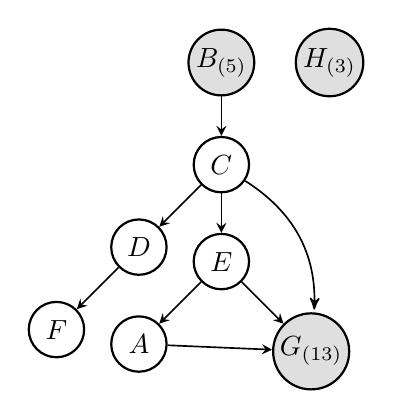
\begin{tikzpicture}[
      nodes={
        draw=black!20, thick, fill=white, font=\normalsize,
        minimum width=2.5em, minimum height=2em
      },
      rounded corners, semithick, >=stealth
      ]

      \node[obs]                 (c2) {$B_{{(5)}}$};
      \node[latent, below=0.5 of c2]   (c3){$C$};
      \node[latent, below=0.5 of c3]   (c5){$E$};
      \node[latent, below left = 0.75 of c3] (c4){$D$};
      \node[latent, below left = 0.75 of c4] (c6){$F$};
      \node[latent, below left = 0.75 of c5] (c1){$A$};
      \node[obs, below right = 0.75 of c5] (c7) {$G_{(13)}$};
      \node[obs, right = 0.5 of c2] (c8){$H_{{(3)}}$};


  % Connect the nodes
  \edge {c2}{c3};
  \edge {c3}{c4,c5};
  \draw[->,>=stealth', shorten >= 1pt] (c3) to[bend left](c7);
  \edge {c4}{c6};
  \edge {c5}{c1,c7};
  \edge {c1}{c7};
  %\edge {p1,p2} {y} ; %
  %\edge {y} {c2} ;
  %\edge {y}{c1};



\end{tikzpicture}
%\endpgfgraphicnamed

%%% Local Variables:
%%% mode: tex-pdf
%%% TeX-master: "example"
%%% End:

  \end{tabular}
  \caption{The Bayesian network obtained with K2 on the prediscretized Auto MPG dataset}
  \label{Auto_graph_1}
\end{figure}

Table \ref{Auto_MPG_disc_table_1} shows the numbers of intervals after discretization, the positions of discretization edges, and log-likelihood of 10-fold cross validation. For the Bayesian network in Fig. \ref{Auto_graph_1}, the approximation only reduces runtime of proposed method and has no influence on discretization result. MDL principle discretization works not well, since it discretizes all variables with only one interval. For a Bayesian network on thie Auto MPG data set that MDL principle discretization has non-trivial result, please reference to Appendix.

\begin{table}[h]
  \centering
  \scriptsize
\begin{tabular}{cccc}
    \toprule
    Var. & Bayesian & Bayesian with Approximation & MDL \\
    \midrule
    $A$ & \numlist[list-final-separator = {, }]{15.25; 17.65; 20.90; 25.65; 28.90} & \numlist[list-final-separator = {, }]{15.25; 17.65; 20.90; 25.65; 28.90} & - \\
    $C$ & \numlist[list-final-separator = {, }]{70.5; 93.5; 109.0; 159.5; 259.0; 284.5} & \numlist[list-final-separator = {, }]{70.5;93.5;109.0;159.5;259.0;284.5} & - \\
    $D$ & \numlist[list-final-separator = {, }]{71.5;99.0;127.0} & \numlist[list-final-separator = {, }]{71.5;99.0; 127.0} & - \\
    $E$ & \numlist[list-final-separator = {, }]{2115;2481;2960;3658} & \numlist[list-final-separator = {, }]{2115;2481;2960;3658} & - \\
    $F$ & \numlist[list-final-separator = {, }]{12.35;13.75;16.05;22.85} & \numlist[list-final-separator = {, }]{12.35;13.75;16.05;22.85} & - \\
    \addlinespace[0.5em]
    Logl & \num{-10210} & \num{-10210} & \num{-11918} \\
    \bottomrule
\end{tabular}
  \caption{Discretization result of Auto MPG dataset based on the graph in Fig. \ref{Auto_graph_1}. The discretization policy for the heuristic matches that for the optimal Bayesian approach. \todo{Need to explain why MDL fails}}
  \label{Auto_MPG_disc_table_1}
\end{table}

Figure \ref{auto_exp1_distr_1_3} compares the discretization result on continuous variables $A$ and $C$ with the raw data of Auto MPG data set. The color of discretized area shows the probability of a sample being in the discretized area. The black dots in Figure \ref{auto_exp1_distr_1_3} demonstrate the distribution of the raw data. As shown in the figure, the discretization edges and the resulting marginalized probability match the raw data very well.

\begin{figure}[ht]
    \begin{tabular}{cc}
      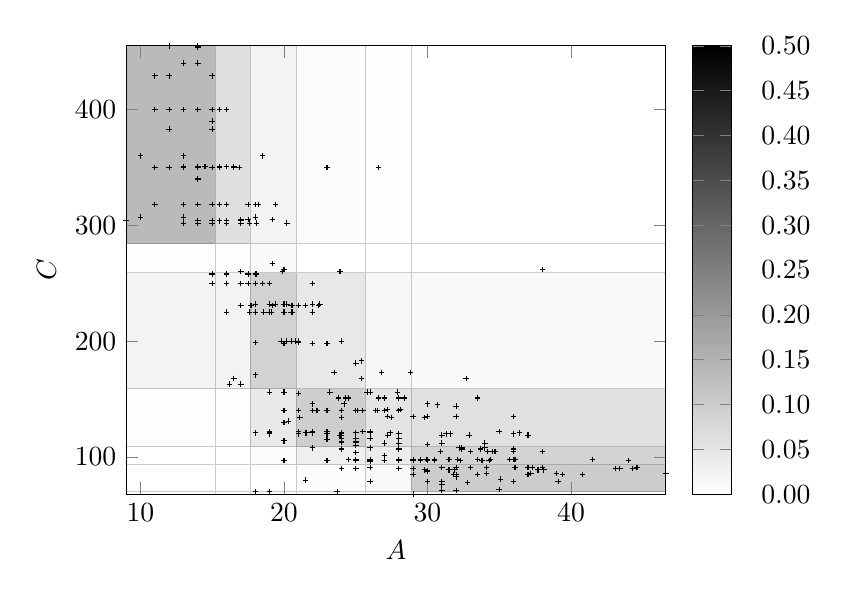
\begin{tikzpicture}
		\begin{axis}[
			view={0}{90},
			enlargelimits=0,
			zmin=0.0, zmax=1.0,
			xlabel=$A$,
			ylabel=$C$,
			colorbar,
			point meta min=0, point meta max=0.5,
			colormap={}{ gray(0cm)=(1); gray(1cm)=(0);},
			colorbar style={
			        ytick={0,0.05,...,0.51},
			        yticklabel style={
			            text width=2.5em,
			            align=right,
			            /pgf/number format/.cd,
			                fixed,
			                fixed zerofill
			        }
			    }
			]

			\addplot3[patch,shader=faceted,patch type=rectangle] coordinates {(9.0000,68.0000,0.0000) (15.2500,68.0000,0.0000) (15.2500,70.5000,0.0000) (9.0000,70.5000,0.0000)};
			\addplot3[patch,shader=faceted,patch type=rectangle] coordinates {(9.0000,70.5000,0.0000) (15.2500,70.5000,0.0000) (15.2500,93.5000,0.0000) (9.0000,93.5000,0.0000)};
			\addplot3[patch,shader=faceted,patch type=rectangle] coordinates {(9.0000,93.5000,0.0000) (15.2500,93.5000,0.0000) (15.2500,109.0000,0.0000) (9.0000,109.0000,0.0000)};
			\addplot3[patch,shader=faceted,patch type=rectangle] coordinates {(9.0000,109.0000,0.0020) (15.2500,109.0000,0.0020) (15.2500,159.5000,0.0020) (9.0000,159.5000,0.0020)};
			\addplot3[patch,shader=faceted,patch type=rectangle] coordinates {(9.0000,159.5000,0.0235) (15.2500,159.5000,0.0235) (15.2500,259.0000,0.0235) (9.0000,259.0000,0.0235)};
			\addplot3[patch,shader=faceted,patch type=rectangle] coordinates {(9.0000,259.0000,0.0030) (15.2500,259.0000,0.0030) (15.2500,284.5000,0.0030) (9.0000,284.5000,0.0030)};
			\addplot3[patch,shader=faceted,patch type=rectangle] coordinates {(9.0000,284.5000,0.1345) (15.2500,284.5000,0.1345) (15.2500,455.0000,0.1345) (9.0000,455.0000,0.1345)};

			\addplot3[patch,shader=faceted,patch type=rectangle] coordinates {(15.2500,68.0000,0.0000) (17.6500,68.0000,0.0000) (17.6500,70.5000,0.0000) (15.2500,70.5000,0.0000)};
			\addplot3[patch,shader=faceted,patch type=rectangle] coordinates {(15.2500,70.5000,0.0000) (17.6500,70.5000,0.0000) (17.6500,93.5000,0.0000) (15.2500,93.5000,0.0000)};
			\addplot3[patch,shader=faceted,patch type=rectangle] coordinates {(15.2500,93.5000,0.0000) (17.6500,93.5000,0.0000) (17.6500,109.0000,0.0000) (15.2500,109.0000,0.0000)};
			\addplot3[patch,shader=faceted,patch type=rectangle] coordinates {(15.2500,109.0000,0.0020) (17.6500,109.0000,0.0020) (17.6500,159.5000,0.0020) (15.2500,159.5000,0.0020)};
			\addplot3[patch,shader=faceted,patch type=rectangle] coordinates {(15.2500,159.5000,0.0230) (17.6500,159.5000,0.0230) (17.6500,259.0000,0.0230) (15.2500,259.0000,0.0230)};
			\addplot3[patch,shader=faceted,patch type=rectangle] coordinates {(15.2500,259.0000,0.0030) (17.6500,259.0000,0.0030) (17.6500,284.5000,0.0030) (15.2500,284.5000,0.0030)};
			\addplot3[patch,shader=faceted,patch type=rectangle] coordinates {(15.2500,284.5000,0.0625) (17.6500,284.5000,0.0625) (17.6500,455.0000,0.0625) (15.2500,455.0000,0.0625)};

			\addplot3[patch,shader=faceted,patch type=rectangle] coordinates {(17.6500,68.0000,0.0000) (20.9000,68.0000,0.0000) (20.9000,70.5000,0.0000) (17.6500,70.5000,0.0000)};
			\addplot3[patch,shader=faceted,patch type=rectangle] coordinates {(17.6500,70.5000,0.0000) (20.9000,70.5000,0.0000) (20.9000,93.5000,0.0000) (17.6500,93.5000,0.0000)};
			\addplot3[patch,shader=faceted,patch type=rectangle] coordinates {(17.6500,93.5000,0.0070) (20.9000,93.5000,0.0070) (20.9000,109.0000,0.0070) (17.6500,109.0000,0.0070)};
			\addplot3[patch,shader=faceted,patch type=rectangle] coordinates {(17.6500,109.0000,0.0430) (20.9000,109.0000,0.0430) (20.9000,159.5000,0.0430) (17.6500,159.5000,0.0430)};
			\addplot3[patch,shader=faceted,patch type=rectangle] coordinates {(17.6500,159.5000,0.0880) (20.9000,159.5000,0.0880) (20.9000,259.0000,0.0880) (17.6500,259.0000,0.0880)};
			\addplot3[patch,shader=faceted,patch type=rectangle] coordinates {(17.6500,259.0000,0.0095) (20.9000,259.0000,0.0095) (20.9000,284.5000,0.0095) (17.6500,284.5000,0.0095)};
			\addplot3[patch,shader=faceted,patch type=rectangle] coordinates {(17.6500,284.5000,0.0225) (20.9000,284.5000,0.0225) (20.9000,455.0000,0.0225) (17.6500,455.0000,0.0225)};

			\addplot3[patch,shader=faceted,patch type=rectangle] coordinates {(20.9000,68.0000,0.0015) (25.6500,68.0000,0.0015) (25.6500,70.5000,0.0015) (20.9000,70.5000,0.0015)};
			\addplot3[patch,shader=faceted,patch type=rectangle] coordinates {(20.9000,70.5000,0.0060) (25.6500,70.5000,0.0060) (25.6500,93.5000,0.0060) (20.9000,93.5000,0.0060)};
			\addplot3[patch,shader=faceted,patch type=rectangle] coordinates {(20.9000,93.5000,0.0320) (25.6500,93.5000,0.0320) (25.6500,109.0000,0.0320) (20.9000,109.0000,0.0320)};
			\addplot3[patch,shader=faceted,patch type=rectangle] coordinates {(20.9000,109.0000,0.0945) (25.6500,109.0000,0.0945) (25.6500,159.5000,0.0945) (20.9000,159.5000,0.0945)};
			\addplot3[patch,shader=faceted,patch type=rectangle] coordinates {(20.9000,159.5000,0.0455) (25.6500,159.5000,0.0455) (25.6500,259.0000,0.0455) (20.9000,259.0000,0.0455)};
			\addplot3[patch,shader=faceted,patch type=rectangle] coordinates {(20.9000,259.0000,0.0000) (25.6500,259.0000,0.0000) (25.6500,284.5000,0.0000) (20.9000,284.5000,0.0000)};
			\addplot3[patch,shader=faceted,patch type=rectangle] coordinates {(20.9000,284.5000,0.0070) (25.6500,284.5000,0.0070) (25.6500,455.0000,0.0070) (20.9000,455.0000,0.0070)};

			\addplot3[patch,shader=faceted,patch type=rectangle] coordinates {(25.6500,68.0000,0.0055) (28.9000,68.0000,0.0055) (28.9000,70.5000,0.0055) (25.6500,70.5000,0.0055)};
			\addplot3[patch,shader=faceted,patch type=rectangle] coordinates {(25.6500,70.5000,0.0110) (28.9000,70.5000,0.0110) (28.9000,93.5000,0.0110) (25.6500,93.5000,0.0110)};
			\addplot3[patch,shader=faceted,patch type=rectangle] coordinates {(25.6500,93.5000,0.0375) (28.9000,93.5000,0.0375) (28.9000,109.0000,0.0375) (25.6500,109.0000,0.0375)};
			\addplot3[patch,shader=faceted,patch type=rectangle] coordinates {(25.6500,109.0000,0.0545) (28.9000,109.0000,0.0545) (28.9000,159.5000,0.0545) (25.6500,159.5000,0.0545)};
			\addplot3[patch,shader=faceted,patch type=rectangle] coordinates {(25.6500,159.5000,0.0165) (28.9000,159.5000,0.0165) (28.9000,259.0000,0.0165) (25.6500,259.0000,0.0165)};
			\addplot3[patch,shader=faceted,patch type=rectangle] coordinates {(25.6500,259.0000,0.0000) (28.9000,259.0000,0.0000) (28.9000,284.5000,0.0000) (25.6500,284.5000,0.0000)};
			\addplot3[patch,shader=faceted,patch type=rectangle] coordinates {(25.6500,284.5000,0.0035) (28.9000,284.5000,0.0035) (28.9000,455.0000,0.0035) (25.6500,455.0000,0.0035)};

			\addplot3[patch,shader=faceted,patch type=rectangle] coordinates {(28.9000,68.0000,0.0030) (46.6000,68.0000,0.0030) (46.6000,70.5000,0.0030) (28.9000,70.5000,0.0030)};
			\addplot3[patch,shader=faceted,patch type=rectangle] coordinates {(28.9000,70.5000,0.0995) (46.6000,70.5000,0.0995) (46.6000,93.5000,0.0995) (28.9000,93.5000,0.0995)};
			\addplot3[patch,shader=faceted,patch type=rectangle] coordinates {(28.9000,93.5000,0.0860) (46.6000,93.5000,0.0860) (46.6000,109.0000,0.0860) (28.9000,109.0000,0.0860)};
			\addplot3[patch,shader=faceted,patch type=rectangle] coordinates {(28.9000,109.0000,0.0605) (46.6000,109.0000,0.0605) (46.6000,159.5000,0.0605) (28.9000,159.5000,0.0605)};
			\addplot3[patch,shader=faceted,patch type=rectangle] coordinates {(28.9000,159.5000,0.0120) (46.6000,159.5000,0.0120) (46.6000,259.0000,0.0120) (28.9000,259.0000,0.0120)};
			\addplot3[patch,shader=faceted,patch type=rectangle] coordinates {(28.9000,259.0000,0.0000) (46.6000,259.0000,0.0000) (46.6000,284.5000,0.0000) (28.9000,284.5000,0.0000)};
			\addplot3[patch,shader=faceted,patch type=rectangle] coordinates {(28.9000,284.5000,0.0005) (46.6000,284.5000,0.0005) (46.6000,455.0000,0.0005) (28.9000,455.0000,0.0005)};

			\addplot3[mark=+, draw=none, mark size=1.0] coordinates {
(18.000,307.000,1) (15.000,350.000,1) (18.000,318.000,1) (16.000,304.000,1) (17.000,302.000,1) (15.000,429.000,1) (14.000,454.000,1) (14.000,440.000,1) (14.000,455.000,1) (15.000,390.000,1) (15.000,383.000,1) (14.000,340.000,1) (15.000,400.000,1) (14.000,455.000,1) (24.000,113.000,1) (22.000,198.000,1) (18.000,199.000,1) (21.000,200.000,1) (27.000,97.000,1) (26.000,97.000,1) (25.000,110.000,1) (24.000,107.000,1) (25.000,104.000,1) (26.000,121.000,1) (21.000,199.000,1) (10.000,360.000,1) (10.000,307.000,1) (11.000,318.000,1) (9.000,304.000,1) (27.000,97.000,1) (28.000,140.000,1) (25.000,113.000,1) (19.000,232.000,1) (16.000,225.000,1) (17.000,250.000,1) (19.000,250.000,1) (18.000,232.000,1) (14.000,350.000,1) (14.000,400.000,1) (14.000,351.000,1) (14.000,318.000,1) (12.000,383.000,1) (13.000,400.000,1) (13.000,400.000,1) (18.000,258.000,1) (22.000,140.000,1) (19.000,250.000,1) (18.000,250.000,1) (23.000,122.000,1) (28.000,116.000,1) (30.000,79.000,1) (30.000,88.000,1) (31.000,71.000,1) (35.000,72.000,1) (27.000,97.000,1) (26.000,91.000,1) (24.000,113.000,1) (25.000,97.500,1) (23.000,97.000,1) (20.000,140.000,1) (21.000,122.000,1) (13.000,350.000,1) (14.000,400.000,1) (15.000,318.000,1) (14.000,351.000,1) (17.000,304.000,1) (11.000,429.000,1) (13.000,350.000,1) (12.000,350.000,1) (13.000,400.000,1) (19.000,70.000,1) (15.000,304.000,1) (13.000,307.000,1) (13.000,302.000,1) (14.000,318.000,1) (18.000,121.000,1) (22.000,121.000,1) (21.000,120.000,1) (26.000,96.000,1) (22.000,122.000,1) (28.000,97.000,1) (23.000,120.000,1) (28.000,98.000,1) (27.000,97.000,1) (13.000,350.000,1) (14.000,304.000,1) (13.000,350.000,1) (14.000,302.000,1) (15.000,318.000,1) (12.000,429.000,1) (13.000,400.000,1) (13.000,351.000,1) (14.000,318.000,1) (13.000,440.000,1) (12.000,455.000,1) (13.000,360.000,1) (18.000,225.000,1) (16.000,250.000,1) (18.000,232.000,1) (18.000,250.000,1) (23.000,198.000,1) (26.000,97.000,1) (11.000,400.000,1) (12.000,400.000,1) (13.000,360.000,1) (12.000,350.000,1) (18.000,232.000,1) (20.000,97.000,1) (21.000,140.000,1) (22.000,108.000,1) (18.000,70.000,1) (19.000,122.000,1) (21.000,155.000,1) (26.000,98.000,1) (15.000,350.000,1) (16.000,400.000,1) (29.000,68.000,1) (24.000,116.000,1) (20.000,114.000,1) (19.000,121.000,1) (15.000,318.000,1) (24.000,121.000,1) (20.000,156.000,1) (11.000,350.000,1) (20.000,198.000,1) (19.000,232.000,1) (15.000,250.000,1) (31.000,79.000,1) (26.000,122.000,1) (32.000,71.000,1) (25.000,140.000,1) (16.000,250.000,1) (16.000,258.000,1) (18.000,225.000,1) (16.000,302.000,1) (13.000,350.000,1) (14.000,318.000,1) (14.000,302.000,1) (14.000,304.000,1) (29.000,98.000,1) (26.000,79.000,1) (26.000,97.000,1) (31.000,76.000,1) (32.000,83.000,1) (28.000,90.000,1) (24.000,90.000,1) (26.000,116.000,1) (24.000,120.000,1) (26.000,108.000,1) (31.000,79.000,1) (19.000,225.000,1) (18.000,250.000,1) (15.000,250.000,1) (15.000,250.000,1) (16.000,400.000,1) (15.000,350.000,1) (16.000,318.000,1) (14.000,351.000,1) (17.000,231.000,1) (16.000,250.000,1) (15.000,258.000,1) (18.000,225.000,1) (21.000,231.000,1) (20.000,262.000,1) (13.000,302.000,1) (29.000,97.000,1) (23.000,140.000,1) (20.000,232.000,1) (23.000,140.000,1) (24.000,134.000,1) (25.000,90.000,1) (24.000,119.000,1) (18.000,171.000,1) (29.000,90.000,1) (19.000,232.000,1) (23.000,115.000,1) (23.000,120.000,1) (22.000,121.000,1) (25.000,121.000,1) (33.000,91.000,1) (28.000,107.000,1) (25.000,116.000,1) (25.000,140.000,1) (26.000,98.000,1) (27.000,101.000,1) (17.500,305.000,1) (16.000,318.000,1) (15.500,304.000,1) (14.500,351.000,1) (22.000,225.000,1) (22.000,250.000,1) (24.000,200.000,1) (22.500,232.000,1) (29.000,85.000,1) (24.500,98.000,1) (29.000,90.000,1) (33.000,91.000,1) (20.000,225.000,1) (18.000,250.000,1) (18.500,250.000,1) (17.500,258.000,1) (29.500,97.000,1) (32.000,85.000,1) (28.000,97.000,1) (26.500,140.000,1) (20.000,130.000,1) (13.000,318.000,1) (19.000,120.000,1) (19.000,156.000,1) (16.500,168.000,1) (16.500,350.000,1) (13.000,350.000,1) (13.000,302.000,1) (13.000,318.000,1) (31.500,98.000,1) (30.000,111.000,1) (36.000,79.000,1) (25.500,122.000,1) (33.500,85.000,1) (17.500,305.000,1) (17.000,260.000,1) (15.500,318.000,1) (15.000,302.000,1) (17.500,250.000,1) (20.500,231.000,1) (19.000,225.000,1) (18.500,250.000,1) (16.000,400.000,1) (15.500,350.000,1) (15.500,400.000,1) (16.000,351.000,1) (29.000,97.000,1) (24.500,151.000,1) (26.000,97.000,1) (25.500,140.000,1) (30.500,98.000,1) (33.500,98.000,1) (30.000,97.000,1) (30.500,97.000,1) (22.000,146.000,1) (21.500,121.000,1) (21.500,80.000,1) (43.100,90.000,1) (36.100,98.000,1) (32.800,78.000,1) (39.400,85.000,1) (36.100,91.000,1) (19.900,260.000,1) (19.400,318.000,1) (20.200,302.000,1) (19.200,231.000,1) (20.500,200.000,1) (20.200,200.000,1) (25.100,140.000,1) (20.500,225.000,1) (19.400,232.000,1) (20.600,231.000,1) (20.800,200.000,1) (18.600,225.000,1) (18.100,258.000,1) (19.200,305.000,1) (17.700,231.000,1) (18.100,302.000,1) (17.500,318.000,1) (30.000,98.000,1) (27.500,134.000,1) (27.200,119.000,1) (30.900,105.000,1) (21.100,134.000,1) (23.200,156.000,1) (23.800,151.000,1) (23.900,119.000,1) (20.300,131.000,1) (17.000,163.000,1) (21.600,121.000,1) (16.200,163.000,1) (31.500,89.000,1) (29.500,98.000,1) (21.500,231.000,1) (19.800,200.000,1) (22.300,140.000,1) (20.200,232.000,1) (20.600,225.000,1) (17.000,305.000,1) (17.600,302.000,1) (16.500,351.000,1) (18.200,318.000,1) (16.900,350.000,1) (15.500,351.000,1) (19.200,267.000,1) (18.500,360.000,1) (31.900,89.000,1) (34.100,86.000,1) (35.700,98.000,1) (27.400,121.000,1) (25.400,183.000,1) (23.000,350.000,1) (27.200,141.000,1) (23.900,260.000,1) (34.200,105.000,1) (34.500,105.000,1) (31.800,85.000,1) (37.300,91.000,1) (28.400,151.000,1) (28.800,173.000,1) (26.800,173.000,1) (33.500,151.000,1) (41.500,98.000,1) (38.100,89.000,1) (32.100,98.000,1) (37.200,86.000,1) (28.000,151.000,1) (26.400,140.000,1) (24.300,151.000,1) (19.100,225.000,1) (34.300,97.000,1) (29.800,134.000,1) (31.300,120.000,1) (37.000,119.000,1) (32.200,108.000,1) (46.600,86.000,1) (27.900,156.000,1) (40.800,85.000,1) (44.300,90.000,1) (43.400,90.000,1) (36.400,121.000,1) (30.000,146.000,1) (44.600,91.000,1) (33.800,97.000,1) (29.800,89.000,1) (32.700,168.000,1) (23.700,70.000,1) (35.000,122.000,1) (32.400,107.000,1) (27.200,135.000,1) (26.600,151.000,1) (25.800,156.000,1) (23.500,173.000,1) (30.000,135.000,1) (39.100,79.000,1) (39.000,86.000,1) (35.100,81.000,1) (32.300,97.000,1) (37.000,85.000,1) (37.700,89.000,1) (34.100,91.000,1) (34.700,105.000,1) (34.400,98.000,1) (29.900,98.000,1) (33.000,105.000,1) (33.700,107.000,1) (32.400,108.000,1) (32.900,119.000,1) (31.600,120.000,1) (28.100,141.000,1) (30.700,145.000,1) (25.400,168.000,1) (24.200,146.000,1) (22.400,231.000,1) (26.600,350.000,1) (20.200,200.000,1) (17.600,225.000,1) (28.000,112.000,1) (27.000,112.000,1) (34.000,112.000,1) (31.000,112.000,1) (29.000,135.000,1) (27.000,151.000,1) (24.000,140.000,1) (36.000,105.000,1) (37.000,91.000,1) (31.000,91.000,1) (38.000,105.000,1) (36.000,98.000,1) (36.000,120.000,1) (36.000,107.000,1) (34.000,108.000,1) (38.000,91.000,1) (32.000,91.000,1) (38.000,91.000,1) (25.000,181.000,1) (38.000,262.000,1) (26.000,156.000,1) (22.000,232.000,1) (32.000,144.000,1) (36.000,135.000,1) (27.000,151.000,1) (27.000,140.000,1) (44.000,97.000,1) (32.000,135.000,1) (28.000,120.000,1) (31.000,119.000,1) };
		\end{axis}
	\end{tikzpicture}

    \end{tabular}
  \caption{Comparison of the raw data and discretization result on variable $A$ and $C$}
  \label{auto_exp1_distr_1_3}
\end{figure}

\subsubsection{Structure is Learned}

If the network structure is not known in advance, it should be learned along with the discretization process. Figure \ref{Auto_graph_2} and Table \ref{Auto_MPG_disc_table_2} show a learned discrete-valued Bayesian network and the corresponding discretization edges of each continuous variable. This result is obtained by running Algorithm \ref{Learn_DBN} fifty times and choosing the one with the highest K2 score.
\newline

 {\centering
\begin{minipage}{0.50\textwidth}
  \centering
  \scalebox{0.7}{
  % model_pca.tex
%
% Copyright (C) 2012 Jaakko Luttinen
%
% This file may be distributed and/or modified
%
% 1. under the LaTeX Project Public License and/or
% 2. under the GNU General Public License.
%
% See the files LICENSE_LPPL and LICENSE_GPL for more details.

% PCA model

%\beginpgfgraphicnamed{model-pca}
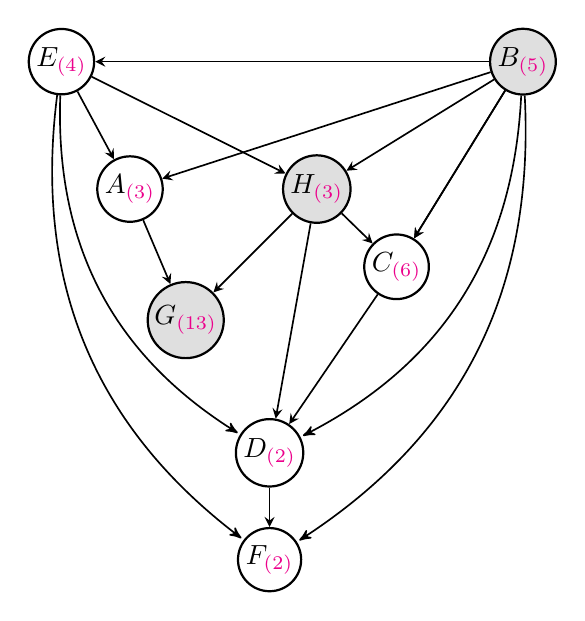
\begin{tikzpicture}[
      nodes={
        draw=black!20, thick, fill=white, font=\normalsize,
        minimum width=2.5em, minimum height=2em
      },
      rounded corners, semithick, >=stealth
      ]

      \node[obs]                 (c2) {$B_{\todo{(5)}}$};
      \node[latent, below left = 2.0 and 1.0 of c2]   (c3){$C_{\todo{(6)}}$};
      \node[latent, left =5.0 of c2]   (c5){$E_{\todo{(4)}}$};
      \node[latent, below left = 1.75 and 1.0 of c3] (c4){$D_{\todo{(2)}}$};
      \node[obs, below left = 1.0 and 2.0 of c2] (c8){$H_{\todo{(3)}}$};
      \node[latent, below = 0.5 of c4] (c6){$F_{\todo{(2)}}$};
      \node[latent, left = 1.5 of c8] (c1){$A_{\todo{(3)}}$};
      \node[obs, below left = 1.0  and 1.0 of c8] (c7) {$G_{\todo{(13)}}$};
      


  % Connect the nodes
  \edge {c2}{c3,c5,c1,c8,c3};
  \draw[->,>=stealth', shorten >= 1pt] (c2) to[bend left](c4);
  \draw[->,>=stealth', shorten >= 1pt] (c2) to[bend left](c6);
  \edge {c5}{c1,c8};
  \draw[->,>=stealth', shorten >= 1pt] (c5) to[bend right](c4);
  \draw[->,>=stealth', shorten >= 1pt] (c5) to[bend right](c6);
  \edge {c8}{c7,c4,c3};
  \edge {c1}{c7};
  \edge {c3}{c4};
  \edge {c4}{c6};
  %\draw[->,>=stealth', shorten >= 1pt] (c3) to[bend left](c7);
  %\edge {c4}{c6};
  %\edge {c5}{c1,c7};
  %\edge {c1}{c7};
  %\edge {p1,p2} {y} ; %
  %\edge {y} {c2} ;
  %\edge {y}{c1};



\end{tikzpicture}
%\endpgfgraphicnamed

%%% Local Variables: 
%%% mode: tex-pdf
%%% TeX-master: "example"
%%% End: 
}
  \captionof{figure}{The learned discrete-\newline valued Bayesian network}
  \label{Auto_graph_2}
\end{minipage}
\begin{minipage}{0.50\textwidth}
  \raggedleft
  \begin{tabular}{|c|c|c|}
\hline
\begin{tabular}[c]{@{}c@{}} Var. \end{tabular} & \begin{tabular}[c]{@{}c@{}}No. of\\ Intvls\end{tabular} & \begin{tabular}[c]{@{}c@{}}Disc.\\ edges\end{tabular}                       \\ \hline
$A$                                                             & 3                                                       & 17.55,23.95                                                                 \\ \hline
$C$                                                             & 6                                                       & \begin{tabular}[c]{@{}c@{}}134.5,159.5,\\ 169.5,259.0,\\ 264.5\end{tabular} \\ \hline
$D$                                                             & 2                                                       & 115.5                                                                       \\ \hline
$E$                                                             & 4                                                       & \begin{tabular}[c]{@{}c@{}}2764.5,\\3030.0,\\ 3923.5\end{tabular}           \\ \hline
$F$                                                             & 2                                                       & 14.05                                                                       \\ \hline
\end{tabular}
  \captionof{table}{The discretization edges of variables in Fig \ref{Auto_graph_2}}
  \label{Auto_MPG_disc_table_2}
\end{minipage}
}

Figure \ref{auto_exp2_distr_1_3} compares the result of Figure \ref{Auto_graph_2} and Table \ref{Auto_MPG_disc_table_2} with the raw data on variables $A$ and $C$. Again, the black dots are raw data points. Although the numbers of discretization edges of $A$ and $C$ shown in Table \ref{Auto_MPG_disc_table_2} are less than Table \ref{Auto_MPG_disc_table_1}, they still have a good capture of raw data distribution.

\begin{figure}[ht]
    \begin{tabular}{cc}
      	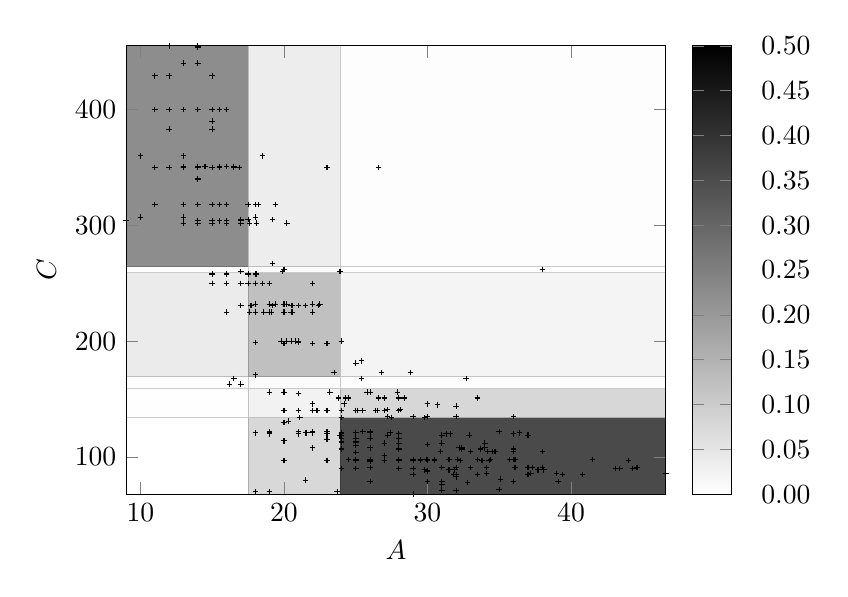
\begin{tikzpicture}
		\begin{axis}[
			view={0}{90},
			enlargelimits=0,
			zmin=0.0, zmax=1.0,
			xlabel=$A$,
			ylabel=$C$,
			colorbar,
			point meta min=0, point meta max=0.5,
			colormap={}{ gray(0cm)=(1); gray(1cm)=(0);},
			colorbar style={
			        ytick={0,0.05,...,0.51},
			        yticklabel style={
			            text width=2.5em,
			            align=right,
			            /pgf/number format/.cd,
			                fixed,
			                fixed zerofill
			        }
			    }
			]

			\addplot3[patch,shader=faceted,patch type=rectangle] coordinates {(9.0000,68.0000,0.0000) (17.5500,68.0000,0.0000) (17.5500,134.5000,0.0000) (9.0000,134.5000,0.0000)};
			\addplot3[patch,shader=faceted,patch type=rectangle] coordinates {(9.0000,134.5000,0.0010) (17.5500,134.5000,0.0010) (17.5500,159.5000,0.0010) (9.0000,159.5000,0.0010)};
			\addplot3[patch,shader=faceted,patch type=rectangle] coordinates {(9.0000,159.5000,0.0010) (17.5500,159.5000,0.0010) (17.5500,169.5000,0.0010) (9.0000,169.5000,0.0010)};
			\addplot3[patch,shader=faceted,patch type=rectangle] coordinates {(9.0000,169.5000,0.0395) (17.5500,169.5000,0.0395) (17.5500,259.0000,0.0395) (9.0000,259.0000,0.0395)};
			\addplot3[patch,shader=faceted,patch type=rectangle] coordinates {(9.0000,259.0000,0.0045) (17.5500,259.0000,0.0045) (17.5500,264.5000,0.0045) (9.0000,264.5000,0.0045)};
			\addplot3[patch,shader=faceted,patch type=rectangle] coordinates {(9.0000,264.5000,0.2220) (17.5500,264.5000,0.2220) (17.5500,455.0000,0.2220) (9.0000,455.0000,0.2220)};

			\addplot3[patch,shader=faceted,patch type=rectangle] coordinates {(17.5500,68.0000,0.0765) (23.9500,68.0000,0.0765) (23.9500,134.5000,0.0765) (17.5500,134.5000,0.0765)};
			\addplot3[patch,shader=faceted,patch type=rectangle] coordinates {(17.5500,134.5000,0.0260) (23.9500,134.5000,0.0260) (23.9500,159.5000,0.0260) (17.5500,159.5000,0.0260)};
			\addplot3[patch,shader=faceted,patch type=rectangle] coordinates {(17.5500,159.5000,0.0085) (23.9500,159.5000,0.0085) (23.9500,169.5000,0.0085) (17.5500,169.5000,0.0085)};
			\addplot3[patch,shader=faceted,patch type=rectangle] coordinates {(17.5500,169.5000,0.1225) (23.9500,169.5000,0.1225) (23.9500,259.0000,0.1225) (17.5500,259.0000,0.1225)};
			\addplot3[patch,shader=faceted,patch type=rectangle] coordinates {(17.5500,259.0000,0.0070) (23.9500,259.0000,0.0070) (23.9500,264.5000,0.0070) (17.5500,264.5000,0.0070)};
			\addplot3[patch,shader=faceted,patch type=rectangle] coordinates {(17.5500,264.5000,0.0355) (23.9500,264.5000,0.0355) (23.9500,455.0000,0.0355) (17.5500,455.0000,0.0355)};

			\addplot3[patch,shader=faceted,patch type=rectangle] coordinates {(23.9500,68.0000,0.3525) (46.6000,68.0000,0.3525) (46.6000,134.5000,0.3525) (23.9500,134.5000,0.3525)};
			\addplot3[patch,shader=faceted,patch type=rectangle] coordinates {(23.9500,134.5000,0.0770) (46.6000,134.5000,0.0770) (46.6000,159.5000,0.0770) (23.9500,159.5000,0.0770)};
			\addplot3[patch,shader=faceted,patch type=rectangle] coordinates {(23.9500,159.5000,0.0020) (46.6000,159.5000,0.0020) (46.6000,169.5000,0.0020) (23.9500,169.5000,0.0020)};
			\addplot3[patch,shader=faceted,patch type=rectangle] coordinates {(23.9500,169.5000,0.0210) (46.6000,169.5000,0.0210) (46.6000,259.0000,0.0210) (23.9500,259.0000,0.0210)};
			\addplot3[patch,shader=faceted,patch type=rectangle] coordinates {(23.9500,259.0000,0.0000) (46.6000,259.0000,0.0000) (46.6000,264.5000,0.0000) (23.9500,264.5000,0.0000)};
			\addplot3[patch,shader=faceted,patch type=rectangle] coordinates {(23.9500,264.5000,0.0035) (46.6000,264.5000,0.0035) (46.6000,455.0000,0.0035) (23.9500,455.0000,0.0035)};

			\addplot3[mark=+, draw=none, mark size=1.0] coordinates {
(18.000,307.000,1) (15.000,350.000,1) (18.000,318.000,1) (16.000,304.000,1) (17.000,302.000,1) (15.000,429.000,1) (14.000,454.000,1) (14.000,440.000,1) (14.000,455.000,1) (15.000,390.000,1) (15.000,383.000,1) (14.000,340.000,1) (15.000,400.000,1) (14.000,455.000,1) (24.000,113.000,1) (22.000,198.000,1) (18.000,199.000,1) (21.000,200.000,1) (27.000,97.000,1) (26.000,97.000,1) (25.000,110.000,1) (24.000,107.000,1) (25.000,104.000,1) (26.000,121.000,1) (21.000,199.000,1) (10.000,360.000,1) (10.000,307.000,1) (11.000,318.000,1) (9.000,304.000,1) (27.000,97.000,1) (28.000,140.000,1) (25.000,113.000,1) (19.000,232.000,1) (16.000,225.000,1) (17.000,250.000,1) (19.000,250.000,1) (18.000,232.000,1) (14.000,350.000,1) (14.000,400.000,1) (14.000,351.000,1) (14.000,318.000,1) (12.000,383.000,1) (13.000,400.000,1) (13.000,400.000,1) (18.000,258.000,1) (22.000,140.000,1) (19.000,250.000,1) (18.000,250.000,1) (23.000,122.000,1) (28.000,116.000,1) (30.000,79.000,1) (30.000,88.000,1) (31.000,71.000,1) (35.000,72.000,1) (27.000,97.000,1) (26.000,91.000,1) (24.000,113.000,1) (25.000,97.500,1) (23.000,97.000,1) (20.000,140.000,1) (21.000,122.000,1) (13.000,350.000,1) (14.000,400.000,1) (15.000,318.000,1) (14.000,351.000,1) (17.000,304.000,1) (11.000,429.000,1) (13.000,350.000,1) (12.000,350.000,1) (13.000,400.000,1) (19.000,70.000,1) (15.000,304.000,1) (13.000,307.000,1) (13.000,302.000,1) (14.000,318.000,1) (18.000,121.000,1) (22.000,121.000,1) (21.000,120.000,1) (26.000,96.000,1) (22.000,122.000,1) (28.000,97.000,1) (23.000,120.000,1) (28.000,98.000,1) (27.000,97.000,1) (13.000,350.000,1) (14.000,304.000,1) (13.000,350.000,1) (14.000,302.000,1) (15.000,318.000,1) (12.000,429.000,1) (13.000,400.000,1) (13.000,351.000,1) (14.000,318.000,1) (13.000,440.000,1) (12.000,455.000,1) (13.000,360.000,1) (18.000,225.000,1) (16.000,250.000,1) (18.000,232.000,1) (18.000,250.000,1) (23.000,198.000,1) (26.000,97.000,1) (11.000,400.000,1) (12.000,400.000,1) (13.000,360.000,1) (12.000,350.000,1) (18.000,232.000,1) (20.000,97.000,1) (21.000,140.000,1) (22.000,108.000,1) (18.000,70.000,1) (19.000,122.000,1) (21.000,155.000,1) (26.000,98.000,1) (15.000,350.000,1) (16.000,400.000,1) (29.000,68.000,1) (24.000,116.000,1) (20.000,114.000,1) (19.000,121.000,1) (15.000,318.000,1) (24.000,121.000,1) (20.000,156.000,1) (11.000,350.000,1) (20.000,198.000,1) (19.000,232.000,1) (15.000,250.000,1) (31.000,79.000,1) (26.000,122.000,1) (32.000,71.000,1) (25.000,140.000,1) (16.000,250.000,1) (16.000,258.000,1) (18.000,225.000,1) (16.000,302.000,1) (13.000,350.000,1) (14.000,318.000,1) (14.000,302.000,1) (14.000,304.000,1) (29.000,98.000,1) (26.000,79.000,1) (26.000,97.000,1) (31.000,76.000,1) (32.000,83.000,1) (28.000,90.000,1) (24.000,90.000,1) (26.000,116.000,1) (24.000,120.000,1) (26.000,108.000,1) (31.000,79.000,1) (19.000,225.000,1) (18.000,250.000,1) (15.000,250.000,1) (15.000,250.000,1) (16.000,400.000,1) (15.000,350.000,1) (16.000,318.000,1) (14.000,351.000,1) (17.000,231.000,1) (16.000,250.000,1) (15.000,258.000,1) (18.000,225.000,1) (21.000,231.000,1) (20.000,262.000,1) (13.000,302.000,1) (29.000,97.000,1) (23.000,140.000,1) (20.000,232.000,1) (23.000,140.000,1) (24.000,134.000,1) (25.000,90.000,1) (24.000,119.000,1) (18.000,171.000,1) (29.000,90.000,1) (19.000,232.000,1) (23.000,115.000,1) (23.000,120.000,1) (22.000,121.000,1) (25.000,121.000,1) (33.000,91.000,1) (28.000,107.000,1) (25.000,116.000,1) (25.000,140.000,1) (26.000,98.000,1) (27.000,101.000,1) (17.500,305.000,1) (16.000,318.000,1) (15.500,304.000,1) (14.500,351.000,1) (22.000,225.000,1) (22.000,250.000,1) (24.000,200.000,1) (22.500,232.000,1) (29.000,85.000,1) (24.500,98.000,1) (29.000,90.000,1) (33.000,91.000,1) (20.000,225.000,1) (18.000,250.000,1) (18.500,250.000,1) (17.500,258.000,1) (29.500,97.000,1) (32.000,85.000,1) (28.000,97.000,1) (26.500,140.000,1) (20.000,130.000,1) (13.000,318.000,1) (19.000,120.000,1) (19.000,156.000,1) (16.500,168.000,1) (16.500,350.000,1) (13.000,350.000,1) (13.000,302.000,1) (13.000,318.000,1) (31.500,98.000,1) (30.000,111.000,1) (36.000,79.000,1) (25.500,122.000,1) (33.500,85.000,1) (17.500,305.000,1) (17.000,260.000,1) (15.500,318.000,1) (15.000,302.000,1) (17.500,250.000,1) (20.500,231.000,1) (19.000,225.000,1) (18.500,250.000,1) (16.000,400.000,1) (15.500,350.000,1) (15.500,400.000,1) (16.000,351.000,1) (29.000,97.000,1) (24.500,151.000,1) (26.000,97.000,1) (25.500,140.000,1) (30.500,98.000,1) (33.500,98.000,1) (30.000,97.000,1) (30.500,97.000,1) (22.000,146.000,1) (21.500,121.000,1) (21.500,80.000,1) (43.100,90.000,1) (36.100,98.000,1) (32.800,78.000,1) (39.400,85.000,1) (36.100,91.000,1) (19.900,260.000,1) (19.400,318.000,1) (20.200,302.000,1) (19.200,231.000,1) (20.500,200.000,1) (20.200,200.000,1) (25.100,140.000,1) (20.500,225.000,1) (19.400,232.000,1) (20.600,231.000,1) (20.800,200.000,1) (18.600,225.000,1) (18.100,258.000,1) (19.200,305.000,1) (17.700,231.000,1) (18.100,302.000,1) (17.500,318.000,1) (30.000,98.000,1) (27.500,134.000,1) (27.200,119.000,1) (30.900,105.000,1) (21.100,134.000,1) (23.200,156.000,1) (23.800,151.000,1) (23.900,119.000,1) (20.300,131.000,1) (17.000,163.000,1) (21.600,121.000,1) (16.200,163.000,1) (31.500,89.000,1) (29.500,98.000,1) (21.500,231.000,1) (19.800,200.000,1) (22.300,140.000,1) (20.200,232.000,1) (20.600,225.000,1) (17.000,305.000,1) (17.600,302.000,1) (16.500,351.000,1) (18.200,318.000,1) (16.900,350.000,1) (15.500,351.000,1) (19.200,267.000,1) (18.500,360.000,1) (31.900,89.000,1) (34.100,86.000,1) (35.700,98.000,1) (27.400,121.000,1) (25.400,183.000,1) (23.000,350.000,1) (27.200,141.000,1) (23.900,260.000,1) (34.200,105.000,1) (34.500,105.000,1) (31.800,85.000,1) (37.300,91.000,1) (28.400,151.000,1) (28.800,173.000,1) (26.800,173.000,1) (33.500,151.000,1) (41.500,98.000,1) (38.100,89.000,1) (32.100,98.000,1) (37.200,86.000,1) (28.000,151.000,1) (26.400,140.000,1) (24.300,151.000,1) (19.100,225.000,1) (34.300,97.000,1) (29.800,134.000,1) (31.300,120.000,1) (37.000,119.000,1) (32.200,108.000,1) (46.600,86.000,1) (27.900,156.000,1) (40.800,85.000,1) (44.300,90.000,1) (43.400,90.000,1) (36.400,121.000,1) (30.000,146.000,1) (44.600,91.000,1) (33.800,97.000,1) (29.800,89.000,1) (32.700,168.000,1) (23.700,70.000,1) (35.000,122.000,1) (32.400,107.000,1) (27.200,135.000,1) (26.600,151.000,1) (25.800,156.000,1) (23.500,173.000,1) (30.000,135.000,1) (39.100,79.000,1) (39.000,86.000,1) (35.100,81.000,1) (32.300,97.000,1) (37.000,85.000,1) (37.700,89.000,1) (34.100,91.000,1) (34.700,105.000,1) (34.400,98.000,1) (29.900,98.000,1) (33.000,105.000,1) (33.700,107.000,1) (32.400,108.000,1) (32.900,119.000,1) (31.600,120.000,1) (28.100,141.000,1) (30.700,145.000,1) (25.400,168.000,1) (24.200,146.000,1) (22.400,231.000,1) (26.600,350.000,1) (20.200,200.000,1) (17.600,225.000,1) (28.000,112.000,1) (27.000,112.000,1) (34.000,112.000,1) (31.000,112.000,1) (29.000,135.000,1) (27.000,151.000,1) (24.000,140.000,1) (36.000,105.000,1) (37.000,91.000,1) (31.000,91.000,1) (38.000,105.000,1) (36.000,98.000,1) (36.000,120.000,1) (36.000,107.000,1) (34.000,108.000,1) (38.000,91.000,1) (32.000,91.000,1) (38.000,91.000,1) (25.000,181.000,1) (38.000,262.000,1) (26.000,156.000,1) (22.000,232.000,1) (32.000,144.000,1) (36.000,135.000,1) (27.000,151.000,1) (27.000,140.000,1) (44.000,97.000,1) (32.000,135.000,1) (28.000,120.000,1) (31.000,119.000,1) };
		\end{axis}
	\end{tikzpicture}
    \end{tabular}
  \caption{Comparison of the raw data and discretization result on variable $A$ and $C$ according to Figure \ref{Auto_graph_2} and Table \ref{Auto_MPG_disc_table_2}}
  \label{auto_exp2_distr_1_3}
\end{figure}


\subsection{Dataset 2: Wine}
\label{subsec:wine}

In this subsection, two experiments are conducted on the Wine dataset from the Irvine repository \citep{Lichman:2013}. This dataset has 178 instances and 14 variables. Only variable $A$ is discrete-valued with cardinality number 3. Again, in the first experiment, the network structure is given. In the second experiment, the network structure is not provided.

\subsubsection{Experiment 1 on Wine dataset}
\label{subsubsec:wine_exp2}

Figure \ref{Wine_graph_1} is obtained by equal-width discretizing each continuous variable into 3 intervals and running K2 1000 times. Table \ref{Wine_disc_table_1} shows a comparison between the proposed method and the MDL principle discretization method. The proposed method is still better than MDL principle discretization in terms of likelihood, although the latter returns non-trivial result in this experiment. Furthermore, the proposed method with the approximation has more intervals after discretization, thus it has a slightly better result. However, as shown in next dataset, the approximation might cut continuous variables into too many intervals. Therefore, the proposed method without the approximation should be still considered a better approach.


\begin{figure}[ht]
    \begin{tabular}{cc}
      % model_pca.tex
%
% Copyright (C) 2012 Jaakko Luttinen
%
% This file may be distributed and/or modified
%
% 1. under the LaTeX Project Public License and/or
% 2. under the GNU General Public License.
%
% See the files LICENSE_LPPL and LICENSE_GPL for more details.

% PCA model

%\beginpgfgraphicnamed{model-pca}
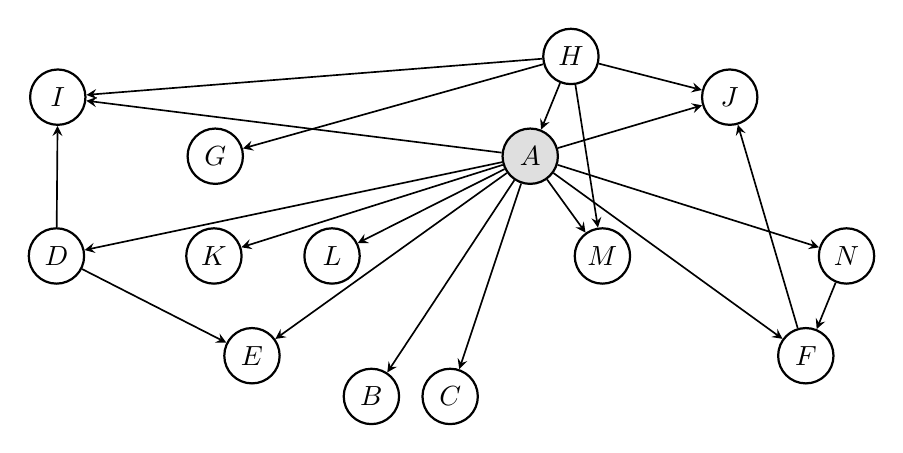
\begin{tikzpicture}[
      nodes={
        draw=black!20, thick, fill=white, font=\normalsize,
        minimum width=2.5em, minimum height=2em
      },
      rounded corners, semithick, >=stealth
      ]

      \node[latent]                 (c8) {$H$};
      \node[obs, below left=0.75 and 0.0 of c8]   (c1){$A$};
      \node[latent, below left=0.75 and 4.0 of c8]   (c7){$G$};
      \node[latent, below right=0.75 and 0.4 of c1] (c13){$M$};
      \node[latent, below right=0.75 and 3.5 of c1] (c14){$N$};
      \node[latent, below left=0.75 and 2.0 of c1] (c12){$L$};
      \node[latent, below left=0.75 and 3.5 of c1] (c11){$K$};
      \node[latent, below left=0.75 and 5.5 of c1] (c4){$D$};
      \node[latent, below left=0.0 and 6.0 of c8] (c9){$I$};
      \node[latent, below left=0.75 and 0.5 of c12] (c5){$E$};
      \node[latent, below left=0.75 and 0.0 of c14] (c6){$F$};
      \node[latent, below right=0.0 and 1.5 of c8] (c10){$J$};
      \node[latent, below right=0.0 and 1.0 of c5] (c2){$B$};   
		\node[latent, below right=0.0 and 2.0 of c5] (c3){$C$};         
      
      %\node[latent, below right = 0.75 and 0.25 of c2] (c5){$5$};
      %\node[latent, below right = 0.75 and 2.0 of c1] (c6) {$6$};
      %\node[latent,below right = 0.75 and 0.5 of c4] (c7){$7$};


  % Connect the nodes
 \edge {c8}{c1,c7,c9,c10,c13};
 \edge {c1}{c4,c11,c12,c2,c3,c14,c13,c9,c10};
 \edge {c1,c4}{c5};
 \edge {c4}{c9};
 \edge {c1,c14}{c6};
 \edge {c6}{c10};
  %\edge {c4}{c7};
  %\draw[->,>=stealth', shorten >= 1pt] (c1) to[bend right](c7);
  %\edge {p1,p2} {y} ; %
  %\edge {y} {c2} ;
  %\edge {y}{c1};



\end{tikzpicture}
%\endpgfgraphicnamed

%%% Local Variables: 
%%% mode: tex-pdf
%%% TeX-master: "example"
%%% End: 

    \end{tabular}
  \caption{K2 structure learning with prediscretization on Wine dataset}
  \label{Wine_graph_1}
\end{figure}

\begin{table}
\centering
\scalebox{1.0}{
\scriptsize
\sisetup{detect-weight = true}
\begin{tabular}{@{}ccc@{}}
\toprule
Variable & Bayesian            & MDL          \\
\midrule
$B$    & \num{12.745}, \num{13.54}                         & \num{12.78}        \\
$C$    & \textbf{\num{1.42}}, \textbf{\num{2.235}}                           & \textbf{\num{1.42}}, \textbf{\num{2.235}}  \\
$D$    & \num{2.03}, \num{2.605}, \num{3.07}               & -            \\
$E$    & \textbf{\num{17.9}}, \num{23.25}                           & \textbf{\num{17.9}}         \\
$F$    & \num{88.5}, \num{135.0}                           & -            \\
$G$    & \num{2.105}, \num{2.58}, \num{3.01}               & -            \\
$H$    & \num{0.975}, \num{1.885}, \num{2.31}, \num{3.355} & -            \\
$I$    & \textbf{\num{0.395}}                                       & \textbf{\num{0.395}}       \\
$J$    & \num{1.185}, \num{1.655}                          & -            \\
$K$    & \textbf{\num{3.46}}, \num{4.85}, \num{7.4}                 & \textbf{\num{3.46}}, \num{7.55}   \\
$L$    & \textbf{\num{0.785}}, \num{1.005}, 1.295                   & \textbf{\num{0.785}}        \\
$M$    & \num{2.475}                                       & \num{2.115}, \num{2.505} \\
$N$    & \num{476.0}, \num{716.0}, \num{900.5}             & -            \\
\addlinespace[0.5em]
Log-Likelihood   & \num{-19.94} & \num{-23.60}        \\
% Logl   & -3550                & -4201        \\
\bottomrule
\end{tabular}
}
\caption{Discretization result of Wine dataset based on the graph Fig. \ref{Wine_graph_1}}
\label{Wine_disc_table_1}
\end{table}



\begin{figure}[ht]
    \begin{tabular}{cc}
      % model_pca.tex
%
% Copyright (C) 2012 Jaakko Luttinen
%
% This file may be distributed and/or modified
%
% 1. under the LaTeX Project Public License and/or
% 2. under the GNU General Public License.
%
% See the files LICENSE_LPPL and LICENSE_GPL for more details.

% PCA model

%\beginpgfgraphicnamed{model-pca}
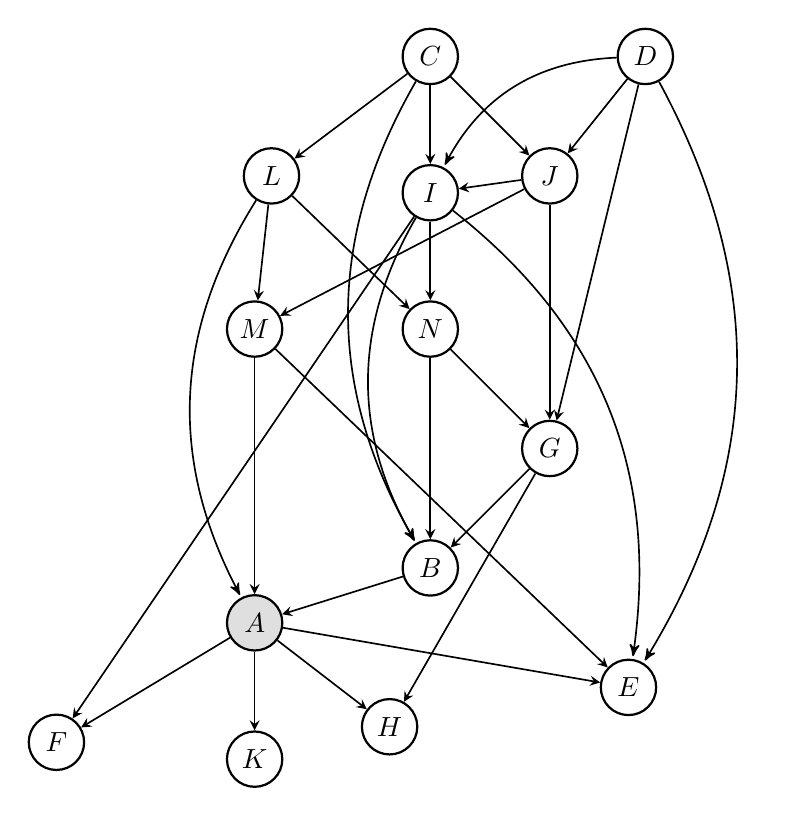
\begin{tikzpicture}[
      nodes={
        draw=black!20, thick, fill=white, font=\normalsize,
        minimum width=2.5em, minimum height=2em
      },
      rounded corners, semithick, >=stealth
      ]

	  \node[latent]          (c3) {$C$};
	  \node[latent, right = 2.0 of c3]  (c4){$D$};
	  \node[latent, below right = 1.0 and 1.0 of c3]  (c10){$J$};
	  \node[latent, below = 1.0 of c3]  (c9){$I$};
	  \node[latent, below = 1.0 of c9]  (c14){$N$};
	  \node[latent, below right = 1.0 and 1.0 of c14] (c7){$G$};
	  \node[latent, below left = 1.0 and 1.0 of c7]  (c2){$B$};
	  \node[latent, below right = 1.0 and 2.0 of c2] (c5){$E$};
	  \node[latent, below left = 1.5 and 0.0 of c2] (c8){$H$};
	  \node[latent, below left = 1.0 and 1.5 of c3] (c12){$L$};
	  \node[latent, left = 1.5 of c14] (c13){$M$};
	  \node[obs, below = 3.0 of c13] (c1){$A$};
	  \node[latent, below = 1.0 of c1] (c11){$K$};
	  \node[latent, below left = 1.0 and 2.0 of c1] (c6){$F$};


  % Connect the nodes

  \edge {c3}{c12,c10,c9};
  \draw[->,>=stealth', shorten >= 1pt] (c3) to[bend right](c2);
  \edge {c4}{c10,c7}
  \draw[->,>=stealth', shorten >= 1pt] (c4) to[bend right](c9);
  \draw[->,>=stealth', shorten >= 1pt] (c4) to[bend left](c5);  
  \edge {c10}{c9,c7,c13};
  \edge{c9}{c14,c6};
  \draw[->,>=stealth', shorten >= 1pt] (c9) to[bend left](c5);
  \draw[->,>=stealth', shorten >= 1pt] (c9) to[bend right](c2);
  \edge {c14}{c2,c7};
  \edge {c7}{c2,c8};
  \edge {c12}{c13,c14};
  \edge {c13}{c1,c5};
  \edge {c1}{c6,c11,c8,c5};
  \edge {c2}{c1};
  \draw[->,>=stealth', shorten >= 1pt] (c12) to[bend right](c1);
  %\draw[->,>=stealth', shorten >= 1pt] (c1) to[bend right](c7);
  %\edge {p1,p2} {y} ; %
  %\edge {y} {c2} ;
  %\edge {y}{c1};



\end{tikzpicture}
%\endpgfgraphicnamed

%%% Local Variables: 
%%% mode: tex-pdf
%%% TeX-master: "example"
%%% End: 

    \end{tabular}
  \caption{K2 structure learning with the proposed discretization method on Wine dataset}
  \label{Wine_graph_2}
\end{figure}


\subsection{Data 3: Housing}
\label{subsec:housing}

\begin{figure}[ht]
    \begin{tabular}{cc}
      % model_pca.tex
%
% Copyright (C) 2012 Jaakko Luttinen
%
% This file may be distributed and/or modified
%
% 1. under the LaTeX Project Public License and/or
% 2. under the GNU General Public License.
%
% See the files LICENSE_LPPL and LICENSE_GPL for more details.

% PCA model

%\beginpgfgraphicnamed{model-pca}
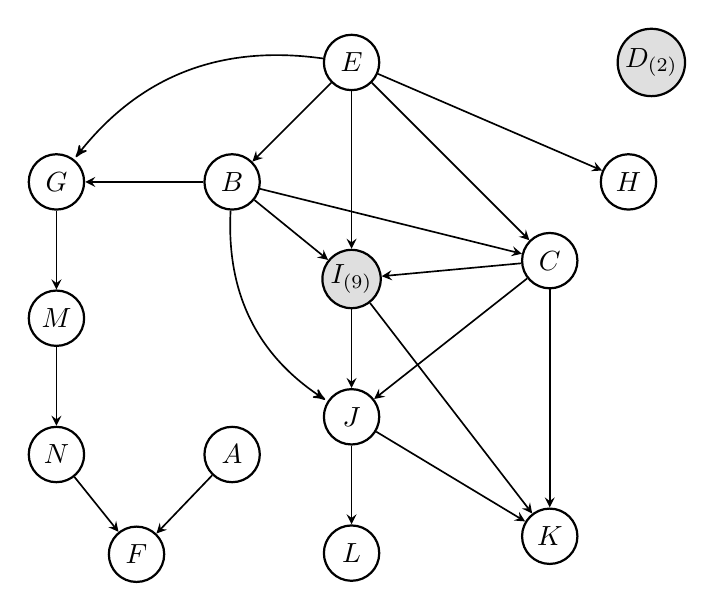
\begin{tikzpicture}[
      nodes={
        draw=black!20, thick, fill=white, font=\normalsize,
        minimum width=2.5em, minimum height=2em
      },
      rounded corners, semithick, >=stealth
      ]

	  \node[latent]          (c5) {$E$};
	  \node[obs, right = 3.0 of c5]  (c4){$D_{{(2)}}$};
	  \node[latent, below left = 1.0 and 1.0 of c5]  (c2){$B$};
	  \node[obs, below = 2.0 of c5]  (c9){$I_{{(9)}}$};
	  \node[latent, below = 1.0 of c9]  (c10){$J$};
	  \node[latent, below = 1.0 of c10] (c12){$L$};
	  \node[latent, below right = 1.0 and 2.0 of c10]  (c11){$K$};
	  \node[latent, below right = 2.0 and 2.0 of c5] (c3){$C$};
	  \node[latent, below right = 1.0 and 3.0 of c5] (c8){$H$};
	  \node[latent, left = 1.5 of c2] (c7){$G$};
	  \node[latent, below = 1.0 of c7] (c13){$M$};
	  \node[latent, below = 1.0 of c13] (c14){$N$};
	  \node[latent, right = 1.5 of c14] (c1){$A$};
	  \node[latent, below right = 0.75 and 0.5 of c14] (c6){$F$};


  % Connect the nodes

  \edge {c5}{c2,c3,c8,c9};
  \draw[->,>=stealth', shorten >= 1pt] (c5) to[bend right](c7);
  \edge {c2}{c9,c3,c7}
  \draw[->,>=stealth', shorten >= 1pt] (c2) to[bend right](c10);
  %\draw[->,>=stealth', shorten >= 1pt] (c4) to[bend left](c5);  
  \edge {c3}{c9,c10,c11};
  \edge{c9}{c10,c11};
  %\draw[->,>=stealth', shorten >= 1pt] (c9) to[bend left](c5);
  %\draw[->,>=stealth', shorten >= 1pt] (c9) to[bend right](c2);
  \edge {c10}{c11,c12};
  \edge {c7}{c13};
  \edge {c13}{c14};
  \edge {c14,c1}{c6};
  %\edge {c1}{c6,c11,c8,c5};
  %\edge {c2}{c1};
  %\draw[->,>=stealth', shorten >= 1pt] (c12) to[bend right](c1);
  %\draw[->,>=stealth', shorten >= 1pt] (c1) to[bend right](c7);
  %\edge {p1,p2} {y} ; %
  %\edge {y} {c2} ;
  %\edge {y}{c1};



\end{tikzpicture}
%\endpgfgraphicnamed

%%% Local Variables: 
%%% mode: tex-pdf
%%% TeX-master: "example"
%%% End: 

    \end{tabular}
  \caption{K2 structure learning with prediscretization on Housing dataset}
  \label{Housing_graph_1}
\end{figure}



\begin{table}
\centering
\scalebox{1.0}{
\begin{tabular}{|c|c|c|c|}
\hline
                                                              & The Proposed Method                                     & \begin{tabular}[c]{@{}c@{}}The Proposed Method\\ With the Approx.\end{tabular} & \begin{tabular}[c]{@{}c@{}}The MDL\\ Discretization\end{tabular} \\ \hline
\begin{tabular}[c]{@{}c@{}}Continuous\\ Variable\end{tabular} & \begin{tabular}[c]{@{}c@{}}No. of\\ Intvls\end{tabular} & \begin{tabular}[c]{@{}c@{}}No. of\\ Intvls\end{tabular}                        & \begin{tabular}[c]{@{}c@{}}No. of\\ Intvls\end{tabular}          \\ \hline
$A$                                                             & 3                                                       & 8                                                                              & 1                                                                \\ \hline
$B$                                                             & 4                                                       & 6                                                                              & 1                                                                \\ \hline
$C$                                                             & 8                                                       & 40                                                                             & 1                                                                \\ \hline
$E$                                                             & 14                                                      & 15                                                                             & 1                                                                \\ \hline
$F$                                                             & 4                                                       & 9                                                                              & 1                                                                \\ \hline
$G$                                                             & 3                                                       & 5                                                                              & 1                                                                \\ \hline
$H$                                                             & 6                                                       & 10                                                                             & 1                                                                \\ \hline
$J$                                                            & 8                                                       & 58                                                                             & 1                                                                \\ \hline
$K$                                                             & 5                                                       & 46                                                                             & 7                                                                \\ \hline
$L$                                                             & 4                                                       & 3                                                                              & 1                                                                \\ \hline
$M$                                                             & 6                                                       & 5                                                                              & 1                                                                \\ \hline
$N$                                                             & 6                                                       & 5                                                                              & 1                                                                \\ \hline
\begin{tabular}[c]{@{}c@{}}log-\\ likelihood\end{tabular}     &  -15886.6364                                            & -14559.4739                                                                    & -2186.4531                                                       \\ \hline
\end{tabular}
}
\caption{Discretization result of Housing dataset based on the graph Fig. \ref{Housing_graph_1}}
\label{Housing_disc_table_1}
\end{table}

\begin{figure}[ht]
    \begin{tabular}{cc}
      % model_pca.tex
%
% Copyright (C) 2012 Jaakko Luttinen
%
% This file may be distributed and/or modified
%
% 1. under the LaTeX Project Public License and/or
% 2. under the GNU General Public License.
%
% See the files LICENSE_LPPL and LICENSE_GPL for more details.

% PCA model

%\beginpgfgraphicnamed{model-pca}
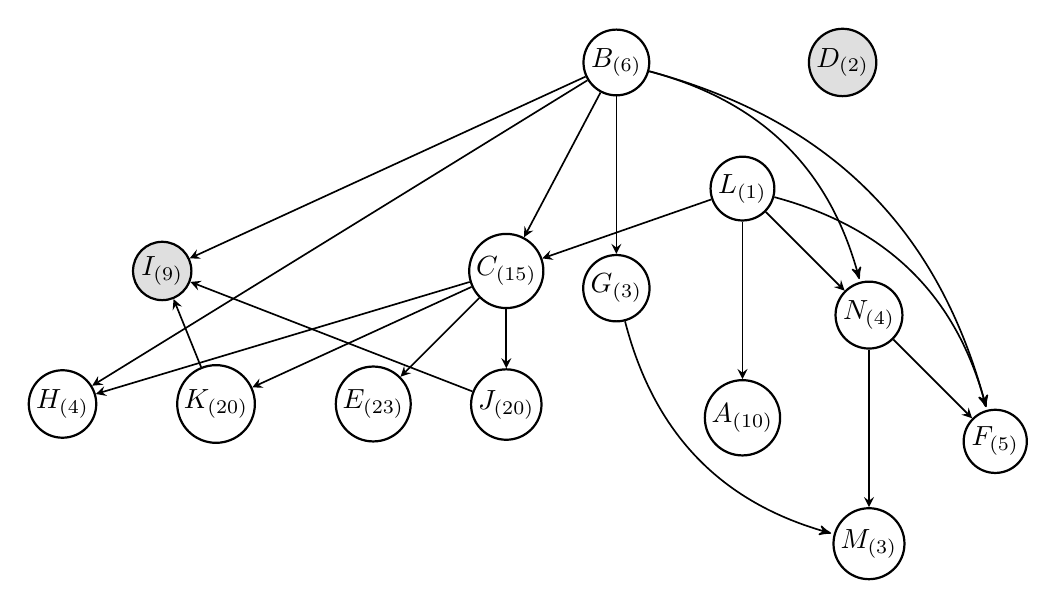
\begin{tikzpicture}[
      nodes={
        draw=black!20, thick, fill=white, font=\normalsize,
        minimum width=2.5em, minimum height=2em
      },
      rounded corners, semithick, >=stealth
      ]

	  \node[latent]          (c2) {$B_{(6)}$};
	  \node[obs, right = 2.0 of c2]  (c4){$D_{(2)}$};
	  \node[latent, below right = 1.0 and 1.0 of c2]  (c12){$L_{(1)}$};
	  \node[latent, below right = 1.0 and 1.0 of c12]  (c14){$N_{(4)}$};
	  \node[latent, below right = 1.0 and 1.0 of c14]  (c6){$F_{(5)}$};
	  \node[latent, below= 2.0 of c2]  (c7){$G_{(3)}$};
	  \node[latent, below = 2.0 of c12]  (c1){$A_{(10)}$};
	  \node[latent, below = 2.0 of c14]  (c13){$M_{(3)}$};
	  \node[latent, below left = 2.0 and 0.75 of c2] (c3){$C_{(15)}$};
	  \node[latent, below = 0.75 of c3]  (c10){$J_{(20)}$};
	  \node[latent, below left = 1.0 and 1.0 of c3] (c5){$E_{(23)}$};
	  \node[latent, left = 1.0 of c5] (c11){$K_{(20)}$};
	  \node[latent, left = 1.0 of c11] (c8){$H_{(4)}$};
	  \node[obs, left = 3.5 of c3] (c9){$I_{(9)}$};

  % Connect the nodes

  \edge {c2}{c9,c8,c3,c7};
  \draw[->,>=stealth', shorten >= 1pt] (c2) to[bend left](c14);
  \draw[->,>=stealth', shorten >= 1pt] (c2) to[bend left](c6);
  \edge {c12}{c3,c1,c14}
  \draw[->,>=stealth', shorten >= 1pt] (c12) to[bend left](c6);
  \edge {c14}{c13,c6}
  \draw[->,>=stealth', shorten >= 1pt] (c7) to[bend right](c13);
  \edge {c3} {c8,c11,c5,c10}
  \edge {c11,c10}{c9}
  %\edge {c2}{c9,c3,c7}
  %\draw[->,>=stealth', shorten >= 1pt] (c2) to[bend right](c10);
  %\draw[->,>=stealth', shorten >= 1pt] (c4) to[bend left](c5);  
  %\edge {c3}{c9,c10,c11};
  %\edge{c9}{c10,c11};
  %\draw[->,>=stealth', shorten >= 1pt] (c9) to[bend left](c5);
  %\draw[->,>=stealth', shorten >= 1pt] (c9) to[bend right](c2);
  %\edge {c10}{c11,c12};
  %\edge {c7}{c13};
  %\edge {c13}{c14};
  %\edge {c14,c1}{c6};
  %\edge {c1}{c6,c11,c8,c5};
  %\edge {c2}{c1};
  %\draw[->,>=stealth', shorten >= 1pt] (c12) to[bend right](c1);
  %\draw[->,>=stealth', shorten >= 1pt] (c1) to[bend right](c7);
  %\edge {p1,p2} {y} ; %
  %\edge {y} {c2} ;
  %\edge {y}{c1};



\end{tikzpicture}
%\endpgfgraphicnamed

%%% Local Variables: 
%%% mode: tex-pdf
%%% TeX-master: "example"
%%% End: 

    \end{tabular}
  \caption{K2 structure learning with the proposed discretization method on Housing dataset}
  \label{Housing_graph_2}
\end{figure}

%%%%%%%%%%%%%%%%%%%%%%%%%%%%%%%%%%%%%%%%%%%%%%%%%%%%%%%%%%%%%%%%%%%%%%%%%%%%%%%%%%%%%%
%\begin{acknowledgements}
%If you'd like to thank anyone, place your comments here
%and remove the percent signs.
%\end{acknowledgements}

% BibTeX users please use one of
%\bibliographystyle{spbasic}      % basic style, author-year citations
%\bibliographystyle{spmpsci}      % mathematics and physical sciences
%\bibliographystyle{spphys}       % APS-like style for physics
%\bibliography{}   % name your BibTeX data base

% Non-BibTeX users please use
%\begin{thebibliography}{}
\bibliographystyle{spbasic}
\bibliography{my_bib}

%%%%%%%%%%%%%%%%%%%%%%%%%%%%%%%%%%%%%%%%%%%%%%%%%%%%%%%%%%%%%%%%%%%%%%%%%%%%%%%%%%%%%%

\section*{Appendices}

\begin{algorithm}
  \caption{ Calculation of $h(u,v)$ for all $u \leq v$}
  \label{alg:h}
  \begin{algorithmic}[1]
  \State Initialize $H$ as an $N \times N$ matrix such that all elements are 0.
  \State $count_p$ is an $N \times N \times \|\Pi_X\|$ matrix such that $count_p [u,v,w]$ is the number of instances from $x_u$ to $x_v$ with $w$th value of $\Pi_X$. This matrix can be calculated in $O(\|\Pi_X\| \cdot N^2)$
  \For {$u = 1$ to $N$}
    \For {$v = u$ to $N$}
      \State $H(u,v) \leftarrow H(u,v) + \log((v-u + J_p)!) - \log((J_p -1)!)$
      \For {$w = 1$ to $\|\Pi_X\|$}
        \State $H(u,v) \leftarrow H(u,v) - \log( count_p(u,v,w)!)$
      \EndFor
    \EndFor
  \EndFor
  \For {$j = 1$ to $n_c$}
    \State \todo{XXX}
  \EndFor
  \end{algorithmic}
\end{algorithm}

\end{document}
% end of file template.tex

